
%============================= HEADER =================================
\chapter{Cosmology}\label{ch:i}

\section{The Cosmological Principle}

Contemporary cosmological models are based on the idea the the Universe is pretty much the same everywhere, a stance sometimes known as the \emph{Copernican Principle} or \emph{Cosmological principle}. If we take it at face value, such a claim seems crazy, if at all logical: There's little resemblance, say, between the center of the Sun (which is kinda hot) and the desolate cold of the ISM\footnote{\emph{Interstellar Medium}.}. The Cosmological Principle starts to make a little more sense if we take it to apply only on the very largest scales, where local variations in density are averaged over and magically disappear.
\begin{figure}[h!]
    \centering 
    \includegraphics[width=0.5\textwidth]{img/isotropyhomogeneity.png}
    \caption{The Cosmological Prinicple automatically translates in two very specific requests: Homogeneity and Isotropy.}
    \label{fgr:homoiso}
\end{figure}
\par The Cosmological principle is related to two more mathematically precise properties that we can request our space-time manifold to have: \emph{Isotropy} and \emph{Homogeneity}, which are given a pictorial representation in Fig.\ref{fgr:homoiso}.
\par Isotropy essentially states that space looks exactly the same around a given point, no matter in what direction you're looking.
\vspace{5pt}
\begin{tcolorbox}[enhanced,attach boxed title to top center={yshift=-3mm,yshifttext=-1mm},
  colback=blue!5!white,colframe=blue!75!black,colbacktitle=blue!80!black,
  title=Isotropy,
  boxed title style={size=small,colframe=blue!50!black}]
  A manifold $M$ is isotropic around a point $p$ if, for any two vectors $V$ and $W$ in the tangent space of $M$ to the point $p$ $T_{p}M$, there is an isometry (symmetry) of $M$ such that the \emph{pushforward} of $W$ under the isometry is parallel with $V$ (not pushed forward). See \cite{carroll}.
\end{tcolorbox}
\par On the other hand, Homogeneity is the statement that the metric is the same throughout the manifold.
\vspace{5pt}
\begin{tcolorbox}[enhanced,attach boxed title to top center={yshift=-3mm,yshifttext=-1mm},
  colback=blue!5!white,colframe=blue!75!black,colbacktitle=blue!80!black,
  title=Homogeneity,
  boxed title style={size=small,colframe=blue!50!black}]
  Given any two points $p$ and $q$ in a manifold $M$, there is an isometry that takes $p$ into $q$. See \cite{carroll}.
\end{tcolorbox}
\par The validity of such principles on the largest scales is manifested in a number of different observations, such as number ounts of galaxies and observations of diffuse X-ray and $\gamma$-ray backgrounds, although it is most clear in the cosmic microwave background (CMB). We're going to spend quite some time with this last lad.
\begin{figure}[h!]
    \centering 
    \includegraphics[width=0.7\textwidth]{img/nhradiosources.png}
    \caption{Dots in the upper part of the figure show the positions of the brightest $4 \cdot 10^{4}$ radio sources visible from the northern hemisphere, and the lower figure shows a comparable number of fainter sources within 15° of the north pole. Their isotropic distribution on the sky confirms that the universe becomes spatially homogeneous on the largest scales.}
    \label{fgr:nhradiosources}
\end{figure}
\par We opened our discussion with a provocative comparison (so to immediately set the unserious tone of these notes), but it's important nonetheless that we ask for ourselves: To what extent is our Universe homogeneous and isotropic?
\par On scales of up to hundreds of Mpc it is not: We see structures in the form of galaxies, clusters of galaxies, filaments and voids.
But on larger scales the Universe does seem to be roughly isotropic. For example, if we counted galaxies in two cubes $100\, \text{Mpc}$ on the side, in opposite directions on the celestial sphere, we would measure the same mean density of matter to within a few percent.
\par As we mentioned, the greatest indicator of the great isotropy (and homogeneity) that reigns in the large-scale Universe is the CMB.

\newpage
\section{The FLRW metric}

In these note, I'll assume you have at least some basic knowledge of GR and/or you are willing to take a look at how the Friedmann, Lemaitre, Robertson, Walker metric is constructed from scratches. So I'm going to present the final result with no proof.
\par If the universe is spatially homogeneous and isotropic at all times, and if distances are allowed to expand or contract as a function of time only\footnote{This is an inevitable consequence of the request of having a metric that is isotropic and homogeneous, for if all points didn't evolve at the same rate, it would be impossible for the Universe to be isotropic.}, the metric is called the FLRW metric:
\begin{equation}
    \text{d}s^{2} = -\text{d}t^{2}+a_{r}(t)^{2}\left(\frac{\text{d}r^{2}}{1-kr^{2}}+r^{2}\text{d}\Omega_{(2)}^{2}\right)
    \label{eq:FRW}
\end{equation}
\par The coordinates used in (\ref{eq:FRW}), in which the metric is free of cross-terms $\text{d}t\text{d}x^{i}$ and the coefficient $\text{d}t^{2}$ is independent of $x^{i}$ are known as \emph{comoving coordinates} and are dimensionless. Xomoving coordinates \emph{do not change at any time}. We can use an alternative form of the metric, obtained by introducing a new radial coordinate $\chi$ defined by
\begin{equation}
    \text{d}\chi = \frac{\text{d}r}{\sqrt{1-kr^{2}}} \implies r = S_{k}(\chi)
    \label{eq:sphere_coordinate}
\end{equation}
where
\begin{equation}
    S_{k}(\chi) = 
    \left\{
    \begin{array}{ll}
        \sin(\chi), & k = +1\\
        \chi, & k = 0\\
        \sinh(\chi), & k = -1
    \end{array}
    \right.
    \label{eq:sphere_radius}
\end{equation}
through which we can write the FLRW metric as
\begin{equation}
    \text{d}s^{2} = -\text{d}t^{2}+a(t)^{2}R_{0}^{2}\left(\text{d}\chi^{2}+S_{k}(\chi)^{2}\text{d}\Omega_{(2)}^{2}\right)
    \label{eq:FRW_revisited}
\end{equation}
The spacelike section of the FLRW metric consists of the spatial metric for a uniformly curves space of radius $R_{0}$ (the present-day radius of curvature) scaled by the square of the scale factor $a(t)$.
\par Note that we're flouting conventional wisdom and adopting a convention in which the scale factor is dimensionless, that requires setting
\begin{equation}
    \bar{r} = R_{0}r \quad \kappa = \frac{k}{R_{0}^{2}} \quad a_{r}(t) = R_{0}a(t)\to a(t)
\end{equation}
thus obtaining a metric with the following form ($\bar{r}\to r$, $\kappa \to k$ for simplicity)
\begin{equation}
    \text{d}s^{2} = -\text{d}t^{2} + a^{2}(t)(\text{d}r^{2}+S_{k}^{2}(r)\text{d}\Omega_{(2)}^{2})
\end{equation}
and the factor $S_{k}(r)$ is simply (\ref{eq:sphere_radius}) scaled with the present-day radius of curvature $R_{0}$. Sometimes it is useful to perform a slight manipulation of the FRW metric (\ref{eq:FRW}) and define a conformal time 
\begin{equation*}
    a(\eta)\text{d}\eta = \text{d}t
\end{equation*}
so that the metric is, guess what, conformal. The scale factor $a$ is therefore factorized and (\ref{eq:FRW_revisited}) becomes
\begin{equation}
    \text{d}s^{2} = a(\eta)^{2}\left(-\text{d}\eta^{2}+\frac{\text{d}r^{2}}{1-kr^{2}}+r^{2}\text{d}\Omega_{(2)}^{2}\right)
    \label{eq:FRW_conf}
\end{equation}
the quantity within parentheses is independent of the conformal time. Since light travels along null geodesics, $\text{d}s^{2} = 0$, the propagation of light in FLRW is the same as in Minkowski space if we first transform to conformal time. Along the path, the change in conformal time equals the change in comoving distance
\begin{equation*}
    \text{d}r = (c)\text{d}\tau \quad \text{d}\Omega = 0
\end{equation*}
The Robertson-Walker metric is an approximation that holds good only on large scales; on smaller scales, the universe is lumpy, and hence does not expand uniformly..
It’s only on scales larger than $\sim 100\,\text{Mpc}$ that the expansion of the Universe can be treated as the ideal, homogeneous, isotropic expansion described by the single scale factor $a(t)$.

\subsection{A short detour on redshift}
In our description of the Universe we'd like to observationally determine a number of quantities to try to infer which of the models proposed by the FRW metric\footnote{As per any GR subject in this notes, I'll follow \cite{carroll}. You can find this discussion at §8.5.}
\begin{equation*}
    \text{d}s^{2} = -\text{d}t^{2}+a(t)^{2}\left(\frac{\text{d}r^{2}}{1-kr^{2}}+r^{2}\text{d}\Omega_{(2)}^{2}\right)
\end{equation*}
corresponds to our Universe. \par We could try with a hand-waving approach and obtain (out of thin air) the expression for the cosmological redshift, but we'll take a somewhat more rigorous approach.
\par Consider the four-velocity of comoving observers $U^{\mu} = (1,0,0,0)$, then the metric admits a Killing tensor of the form 
\begin{equation*}
    K_{\mu\nu} = a^{2}(g_{\mu\nu}+U_{\mu}U_{\nu})
\end{equation*}
that you can check that it satisfies $D_{(\sigma}K_{\mu\nu)} = 0$ where $D_{\sigma}$ is the covariant derivative. By definition of Killing vector (the generalization to a K. tensor is straightforward), the quantity 
\begin{equation}
    K^{2} = K_{\mu\nu}V^{\mu}V^{\nu} = a^{2}\left[V_{\mu}V^{\mu}+(U_{\mu}V^{\mu})^{2}\right]
    \label{eq:conserved_killing}
\end{equation}
is conserved along the geodesics. Here $V^{\mu} = \text{d}x^{\mu}/\text{d}\lambda$. For massive particles, since $V_{\mu}V^{\mu} = -1$ (note the convention on the signature of the metric), we also have
\begin{equation*}
    (V^{0})^{2} = 1+|\vec{V}|^{2} \quad |\vec{V}|^{2} = g_{ij}V^{i}V^{j}
\end{equation*}
Recalling the formula for the four-velocity of the observer, we have $U_{\mu}V^{\mu} = -V^{0}$, so (\ref{eq:conserved_killing}) implies
\begin{equation*}
    |\vec{V}| = \frac{K}{a}
\end{equation*}
Notice how this means that the particle "slows down" with respect to the comoving coordinates as the Universe expands. If we instead consider null geodesics (that is what we're actually interested in)
\begin{equation*}
    V_{\mu}V^{\mu} = 0 \implies U_{\mu}V^{\mu} = \frac{K}{a}
\end{equation*}
but for null-like particles, like photons, we can write the four-velocity as $V^{\mu} = (\omega, \vec{k})$. So the frequency of the photon as measured by a comoving observer is $\omega = -U_{\mu}V^{\mu}$ (remember that $c=1$). The frequency emitted will still be given by the same functional expression but calculated in the local inertial frame of the emitter, so $\omega_{em} = -K/a_{em}$. We then find out that 
\begin{equation*}
    \frac{\omega_{obs}}{\omega_{em}} = \frac{a_{em}}{a_{obs}}
\end{equation*}
To make things easier we then define a quantity called \emph{redshift} defined as 
\begin{equation}
    z_{em} = \frac{\lambda_{obs}-\lambda_{em}}{\lambda_{em}}
    \label{eq:redshift_def}
\end{equation}
so that, if the observation takes place today ($a_{obs} = a_{0} = 1$), we can just write 
\begin{equation}
    \boxed{
    a_{em} = \frac{1}{1+z_{em}}
    }
    \label{eq:scalefactor_redshift}
\end{equation}
and 
\begin{equation}
    \boxed{
    \frac{\nu_{obs}}{\nu_{em}} = \frac{1}{1+z_{em}}
    }
    \label{eq:cosmological_redshift}
\end{equation}
\par Let's give an example. If we observe a galaxy with a redshift $z = 2$, we are observing it as it was when the universe had a scale factor $a(t_{e}) = 1/3$.
\par The redshift we observe for a distant object thus depends only on the relative scale factors at the time of emission and the time of observation. It doesn't depend on how the transition between $a(t_{e})$ and $a(t_{0})$ was made: All that matters is the scale factors at the time of emission and the time of observation.
\par It may be useful to know how to "compose" redshifts. Assume to measure the redshift $z_{1}$ of a distant object when you are yourself on a certain object with redshift $z_{2}$, the "total" redshift that you're going to measure is
\begin{equation}
    1+z_{f} = \frac{a(t_{1})}{a(t_{2})} = \frac{1+z_{2}}{1+z_{1}}
    \label{eq:redshif_comp}
\end{equation}
\par So the redshift tells us two things: The scale factor of the universe when the photon was emitted and, in a sense, the distance of the emitter when the photon was emitted.
\begin{figure}[h!]
    \centering 
    \includegraphics[width=0.7\textwidth]{img/10_1086_320638_fg4_hr.png}
    \caption{A plot of velocity against distance made by \cite{2001ApJ...553...47F}. The different colours represent different ways of measuring distance. The gradient of this line is the \emph{Hubble constant} $H_{0}\sim 72 \,\text{km}\,\text{s}^{-1}\,\text{Mpc}^{-1}$ for these data, as shown by the solid red line.}
\end{figure}
\par Using Hubble's law (assuming we've somehow computed the Hubble constant at its present value) we can easily calculate the \emph{instantaneous physical distance}
\begin{equation*}
    v = cz = H_{0}d_{P}
\end{equation*}
\par Although it's a useful meter of comparison to understand what we're talking about, cosmological redshift has \emph{nothing to do} with a Doppler shift. In fact, even if the Universe was in an age in which $\dot{a} = 0$ and so that $H_{0} = 0$, you wouldn't be able to interpret the shift in frequency as the effect of a Doppler shift ($v = 0$ after all), yet you'd still observe the shift, since $a(t) \neq 0$.
\par However, if we tried to measure $H_{0}$ by finding distances and velocities of galaxies in the direction of Virgo\footnote{The supercluster, not the interferometer.}, we would
be underestimating the Hubble constant, because Virgo-centric inflow partially cancels out the cosmic expansion. Similarly, if we observe galaxies in the opposite direction, our value for $H_{0}$ would be too high. If we correct our observations for this phenomenon, we'd find what's shown in Fig.\ref{fgr:virgoinfall}.
\begin{figure}[h!]
    \centering
    \includegraphics[width=0.7\textwidth]{img/LG_peculiarmotion.png}
    \caption{Diamonds show average recession speed $V_{r}$, measured relative to the Local Group. The two largest white symbols are two clumps within the Virgo cluster; others decrease in size to show distance from Virgo. Left, velocity $V_{r}$ falls further below the linear trend the closer the group is to Virgo; right, after correction for Virgocentric infall. Credits: J. Tonry.}
    \label{fgr:virgoinfall}
\end{figure}

\subsection{Proper distance}

Ignoring the angular dependence, i.e. a point object for which $\text{d}\Omega = 0$, the proper distance between the observer at the origin $r = 0$ and a galaxy at $(r,\theta,\phi)$ can be found using the FLRW metric at a fixed time $t$
\begin{equation*}
    \text{d}s^{2} = a^{2}(t)\text{d}r^{2}
\end{equation*}
so that integrating over the radial comoving distance yields
\begin{equation}
    d_{p}(r) = a(t)\int_{0}^{r}\text{d}r = a(t)r
    \label{eq:properdistance}
\end{equation}
The rate of change for the proper distance between us and a distant galaxy is 
\begin{equation*}
    \dot{d}_{p} = \dot{a}(t)r = \frac{\dot{a}(t)}{a(t)}d_{p} := H(t)d_{p}
\end{equation*}
and we've found the celebrated Hubble law.
\par Let us now approximate $a(t)$ in a neighborhood of today
\begin{equation*}
    a(t) = a(t_{0}) + \left(\parder{a}{t}\right)_{t_{0}}(t-t_{0}) + \frac{1}{2}\left(\parparder{a}{t}\right)_{t_{0}}(t-t_{0})^{2} + \text{o}\left((t-t_{0})^{3}\right)
\end{equation*}
so that ($a(t_{0}) = 1$)
\begin{equation}
    a(t) = 1 + H_{0}(t-t_{0})-\frac{1}{2}q_{0}H_{0}^{2}(t-t_{0})^{2} + \text{o}\left((t-t_{0})^{3}\right)
    \label{eq:a_expansion}
\end{equation}
where we've defined 
\begin{equation}
    H_{0} = \left(\frac{\dot{a}(t)}{a(t)}\right)_{t_{0}} \quad q_{0} = -\left(\frac{\ddot{a}(t)a(t)}{\dot{a}^{2}(t)}\right)_{t_{0}}
    \label{eq:expansion_param}
\end{equation}
so that if $q_{0} > 0$, then $\ddot{a} < 0$ and the expansion of the Universe decelerate. Conversely, if $q_{0} < 0$, then $\ddot{a} > 0$ and the expansion of the Universe accelerate. Recent measurements of $q_{0}$ \cite{Riess_2022} have set
\begin{equation}
    q_{0} = -0.510 \pm 0.024
    \label{eq:acceleration_param}
\end{equation}
\par To determine the value of $H_{0}$ without having to worry about Virgocentric flow and other peculiar velocities, we need to determine the luminosity distance (see below) to standard candles with $d_{l} > 100\,\text{Mpc}$,or $z > 0.02$. But we cannot go too far! At a redshift $z = 0.1$,for instance,the relation between $d_{l}$ (and $d_{p}$) and $z$ starts to deviate significantly from the linear relation that holds true at lower redshifts. To determine the acceleration of the Universe and other cosmological parameters beyond $H_{0}$ we'll have to go farther than that. Indeed, we ought to observe standard candles for which the relation between $d_{l}$ and $z$ deviates significantly from the linear relation that holds true at lower redshifts.
\par Using (\ref{eq:a_expansion}) in the proper distance definition, we can now calculate
\begin{equation}
    d_{p}(t_{0}) = \int_{t_{e}}^{t_{0}} \frac{c\,\text{d}t}{a(t)} \approx c(t_{0}-t_{e}) + \frac{cH_{0}}{2}(t_{0}-t_{e})^{2}
\end{equation}
\par But we also know that
\begin{equation*}
    z = \frac{1}{a(t_{e})}-1
\end{equation*}
so we can find an approximate relation for the redshift
\begin{equation*}
    z \approx H_{0}(t_{0}-t_{e})+\left(1+\frac{q_{0}}{2}\right)H_{0}^{2}(t_{0}-t_{e})^{2}
\end{equation*}
which we can put into the equation for proper distance up to second order in redshift
\begin{equation}
    d_{p}(t_{0}) = \frac{c}{H_{0}}z\left[1-\frac{(1+q_{0})}{2}z\right]
    \label{eq:properdistance_rs_second}
\end{equation}
This tells us something really important: $d_{p}(t_{0})$ is proportional to $z$ only if
\begin{equation*}
    z \ll \frac{2}{1+q_{0}}
\end{equation*}
In this case the proper distance to a galaxy of moderate redshift ($z \sim 0.1$, equivalent of $\sim 400 \,\text{Mpc}$) is less than would be predicted from the
linear Hubble relation.

\subsection{Luminosity Distance}

If the redshift is not very small, we have to think more carefully about what we mean by "distance" in cosmology. The instantaneous physical distance (proper distance) is a convenient construct, but not itself observable, since observation always refer to our past light cone. In Euclidean space, there are a number of different ways to infer the distance of an object, for example comparing its apparent brightness to its intrinsic luminosity.
\par Let us then define the \emph{luminosity distance} as
\begin{equation*}
    d_{l} = \left(\frac{L}{4\pi F}\right)^{1/2}
\end{equation*}
with intrisic luminosity $L$ and $F$. How does this change in a curved and expanding Universe?
\par We can set the comoving radial distance to $r_{e}$, so that photons emitted by and object at this distance will pass (today) through a spehre of proper radius $R = a(t_{0})r_{e} = r_{e}$. The area of such sphere at fixed time can be derived from the coefficient of $\text{d}\Omega$ in (\ref{eq:FRW_revisited}), yielding
\begin{equation*}
    A(t_{0}) = 4\pi R_{0}^{2}S_{k}^{2}(\chi) = 4\pi S_{k}^{2}(r_{e})
\end{equation*}
\par Because of the expansion the wavelength of these photons will change according to (\ref{eq:redshift_def}). Therefore, the energy of a photon will decrease
\begin{equation*}
    E_{0} \sim \frac{c}{\lambda_{0}} = \frac{c}{(1+z)\lambda_{e}} \sim \frac{E_{e}}{1+z}
\end{equation*}
\par On top of that, two wavefronts separated by $\delta t_{e}$ will arrive with a delay $\delta t_{0} = \delta t_{e}(1+z)$, so the arrival rate will decrease of another $1+z$
\begin{equation*}
    L_{e} \sim \frac{E_{e}}{\delta t_{e}} = \frac{(1+z)^{2}E_{0}}{\delta t_{0}} = (1+z)^{2}L_{0}
\end{equation*}
\par Since the flux is equal to energy per unit time per unit area, we can write
\begin{equation*}
    F = \frac{L_{e}}{4\pi S_{k}^{2}(r_{e})(1+z)^{2}}
\end{equation*}
so that by direct comparison with out initial equation, we find that the \emph{luminosity distance} is
\begin{equation}
    d_{l} = S_{k}(r_{e})(1+z) = (1+z)R_{0}S_{k}(\chi)
    \label{eq:luminositydistance}
\end{equation}
\begin{figure}[h!]
    \centering
    \includegraphics[width = 0.8\textwidth]{img/lumdist.png}
    \caption{Luminosity distance of a standard candle with observed redshift $z$, in units of the Hubble distance, $c/H_{0}$. The bold solid line gives the result for the Benchmark Model. For comparison, the dot-dash line indicates a flat, $\Lambda$-dominated Universe, and the dotted line a flat, matter-dominated Universe.}
    \label{fgr:luminosity_dist}
\end{figure}
\par The luminosity distance is something we might hope to measure, sincere there are some astrophysical sources whose absolute luminosity are known (see Chapter \ref{ch:ii}), but $\chi$ (and for extension, the comoving distance $r_{e}$), is not observable, so we have to remove it from our equation. On a null radial geodesic (for convenience), we have
\begin{equation*}
    0 = \text{d}s^{2} = -\text{d}t^{2} + a^{2}R_{0}^{2}\text{d}\chi^{2}
\end{equation*}
or more simply 
\begin{equation*}
    \chi = R_{0}^{-1} \int \frac{\text{d}t}{a} = R_{0}^{-1} \int \frac{\text{d}a}{a^{2}H(a)}
\end{equation*}
\par It is conventional to convert the scale factor to redshift using (\ref{eq:scalefactor_redshift}) $a = (1+z)^{-1}$, so we have
\begin{equation*}
    \chi(z) = R_{0}^{-1}\int_{0}^{z}\frac{\text{d}z'}{H(z')}
\end{equation*}
\par In order to evaluate the Hubble parameter in this integral we can use, as we'll see, the Friedmann equation (\ref{eq:friedmann_alt}), thus finding 
\begin{equation*}
    d_{l}(z) = (1+z)R_{0}S_{k}\left[R_{0}^{-1}H_{0}^{-1}\int \frac{\text{d}z'}{E(z')}\right]
\end{equation*}
where we've defined $E(z) = H(z)/H_{0}$. Note that $R_{0}$ drops out when $k = 0$, which is good, because in that case (flat Universe) the radius of curvature is a completely arbitrary parameter. Still, it is more common to speak in terms of $\Omega_{c,0} = -k/R_{0}^{2}H_{0}^{2}$, which can be measured. In terms of this parameterm we have
\begin{equation*}
    R_{0} = \frac{H_{0}^{-1}}{\sqrt{|\Omega_{c,0}|}}
\end{equation*}
\par We can therefore write the luminosity in terms of measurable cosmological parameters as 
\begin{equation}
    \boxed{
    d_{l}(z) = (1+z)\frac{H_{0}^{-1}}{\sqrt{|\Omega_{c,0}|}}S_{k}\left[\sqrt{|\Omega_{c,0}|}\int \frac{\text{d}z'}{E(z')}\right]
    }
    \label{eq:general_lumdist}
\end{equation}
\par Although it appears unwieldy (and it is), this equation is of central importance in cosmology. Given the observables $H_{0}$ and $\Omega_{i,0}$, we can straightforwardly calculate the luminosity distance to an object at any redshift $z$.
\par Let us now consider a simple case for which we can find a solution right away. If the Universe is roughly flat $S_{k}(r_{e}) \approx r_{e} \approx d_{p}(t_{0})$. Plugging in the second order expansion for the proper distance (\ref{eq:properdistance_rs_second}) into (\ref{eq:luminositydistance}) we find
\begin{equation}
    d_{l}(t_{0}) = \frac{c}{H_{0}}z\left[1+\frac{(1-q_{0})}{2}z\right]
    \label{eq:lumdistance_rs_second}
\end{equation}
\par This relation we could in principle express in terms of apparent and absolute magnitude
\begin{equation*}
    M-m = -5\log_{10}\left(\frac{d_{l}}{1\,\text{Mpc}}\right)-25
\end{equation*}

\subsection{Angular diameter distance}

\par Let's consider a curved, expanding Universe described by the FLRW metric and choose your comoving coordinate system so that you are at the origin.
\par Consider a yardstick of constant proper length $l$ perpendicular to the line of sight and at a comoving coordinate distance $r_{e}$. At a time $t_{e}$, the yardstick emitted the light that you observe at time $t_{0}$. The comoving coordinates of the two ends of the yardstick, at the time the light was emitted, were $(r_{e},\theta_{1},\phi)$ and
$(r_{e},\theta_{2},\phi)$.
\par The distance $\text{d}s$ between the two ends of the yardstick, measured at the time $t_{e}$ when the light was emitted, can be found from the FLRW metric:
\begin{equation*}
    \text{d}s = a(t_{e})S_{k}(r_{e})\delta\theta
\end{equation*}
with $\delta\theta$ the angular distance between the ends of the yardstick. We can set $\text{d}s = l$ and define
\begin{equation}
    d_{a} := \frac{l}{\delta\theta} = \frac{S_{k}(r_{e})}{1+z} = \frac{d_{L}}{(1+z)^{2}}
    \label{eq:angulardistance}
\end{equation}

\subsection{Particle Horizon}

Consider a photon emitted by a galaxy at time $t_{e}$, for a light path $\text{d}s = 0$. The comoving distance traveled at time $t_{x}$ is
\begin{equation*}
    \int_{t_{e}}^{t_{x}} \frac{c\text{d}t}{a(t)} = \int_{0}^{r}\text{d}r = r
\end{equation*}
so that if a photon was emitted at $t_{e} = 0$, the proper distance travelled by the photon is 
\begin{equation}
    d_{H}(t) = a(t)r = a(t)\int_{0}^{t}\frac{c\text{d}t'}{a(t')}
    \label{eq:particle_horizon}
\end{equation}
This has a simple interpretation: The most distant object you can see today is one for which the light emitted at $t = 0$ is just now reaching us at $t = t_{0}$. The proper distance (at the time of observation) to such an object is called the \emph{particle horizon distance}. The particle horizon is a spherical surface centered on you, beyond which you cannot see because light from more distant objects has not had time to reach you.
\par On a concluding note, let us define $r_{H} = c/H(t)$ as the \emph{Hubble radius}. It is the distance at which the expansion rate is faster than the speed of light. The Hubble radius is the distance over which particles can travel in the course of one expansion time.
\par The Hubble radius is a kind of “instantaneous horizon”; it is not fixed in time and does not necessarily mean those points never have been or never will be in causal contact. The Hubble radius evolves as the universe expands or contracts (i.e., $H$ changes).
\par If particles are separated by distances greater than particle horizon, they never could have communicated with one another; if they are separated by distances greater than the Hubble radius, they cannot talk to each other at the time $t$.

\subsubsection{Olbers' paradox and its solution}

Should I ever feel like it, I'll talk about it. At present day (\today), I'm not definitely feeling like it.

\newpage
\section{Friedmann's Equations}

The FLRW metric (\ref{eq:FRW}) is defined for any behavior of the scale factor $a(t)$; the next step would be to plug it into Einstein's equation
\begin{equation}
    G_{\mu\nu} = R_{\mu\nu}-\frac{1}{2}Rg_{\mu\nu} = 8\pi G T_{\mu\nu}
    \label{eq:einstein_eq}
\end{equation}
to derive the so called \emph{Friedmann's equations}. We will chose to model matter and energy by a perfect fluid. This means that is we consider a fluid at rest in the comoving coordinates, then $u^{\mu} = (1,0,0,0)$ and the energy momentum tensor associated to the fluid will be
\begin{equation}
    T_{\mu\nu} = (p+\rho)u_{\mu}u_{\nu} +pg_{\mu\nu} \quad T = -\rho +3p
    \label{eq:perfectfluid}
\end{equation}
\par It is educational to consider the 0th component of the conservation of energy equation
\begin{equation}
    0 = \nabla_{\mu}T^{\mu}_{\; \;0} = -\partial_{0}\rho-3\frac{\ddot{a}}{a}(\rho+p)
    \label{eq:fluidequation}
\end{equation}
which is sometimes known \emph{fluid equation}. Here $\rho$ is the energy density and $p$ is the pressure. Please note that we're working in units $c=1$.
\par Making use of the expressions you can find in the appendix, we can solve explicitly (\ref{eq:einstein_eq}) and find
\begin{equation}
    \boxed{
    \left(\frac{\dot{a}}{a}\right)^{2} = \frac{8\pi G}{3}\rho -\frac{k}{a^{2}}
    }
    \label{eq:friedmann1}
\end{equation}
and 
\begin{equation}
    \boxed{
        \frac{\ddot{a}}{a} = -\frac{4\pi G}{3}(\rho + 3p)
    }
    \label{eq:friedmann2}
\end{equation}
\par If we know the dependence of $\rho$ on the scale factor $a$, the first one (\ref{eq:friedmann1}) is enough to solve for $a$.
\par A useful quantity to introduce is the \emph{density parameter}
\begin{equation}
    \boxed{
        \Omega = \frac{8\pi G}{3H^{2}}\rho = \frac{\rho}{\rho_{c}}
    }
    \label{eq:densityparam}
\end{equation}
where the \emph{critical density} is defined by
\begin{equation}
    \rho_{c} = \frac{3H^{2}}{8\pi G}
\end{equation}
\par Knowing the Hubble constant to within about 1\%, we can predict the current value of the critical density to within about 2\%. TOday, the critical energy density is
\begin{equation}
    \rho_{c}(t_{0}) = \frac{3H_{0}^{2}}{8\pi G} = 4900 \pm 300\,\text{MeV}\,\text{m}^{-3}
\end{equation}
\par This quantity, that will generally change with time, is called the critical density because the Friedmann equation (\ref{eq:friedmann1}) can be written as
\begin{equation}
    \Omega - 1 = \frac{k}{H^{2}a^{2}}
    \label{eq:densityparam_eq}
\end{equation}
that univocally determinates the sign of $k$ depending on whether $\Omega$ is greater then, equal to, or less than, one.
\begin{align*}
    & \rho < \rho_{c} \iff \Omega < 1 \iff k < 0 \iff \text{open} \\
    & \rho = \rho_{c} \iff \Omega = 1 \iff k = 0 \iff \text{flat} \\
    & \rho > \rho_{c} \iff \Omega > 1 \iff k > 0 \iff \text{closed} 
\end{align*}
The density parameter, then, tells us which of the three FLRW geometries describes our Universe. Since the right-hand side of (\ref{eq:densityparam_eq}) cannot change sign as the Universe expands, neither can the left-hand side. So, $\Omega$ will have the same sign \emph{at all times}.
\par The current value of the density parameter, determined from a combination of observational data, lies in the range $0.995<\Omega(t_{0})<1.005$ (2017), while the Planck collaboration along with observations of the BAO\footnote{\emph{Baryonic Acoustic Oscillations}.} set a narrower limit $\Omega(t_{0}) = 0.999 \pm 0.002$, suggesting that the Universe is, indeed, critical.
\par Let us now dedicate a little of our time to find an expression able to predict the temporal evolution of $a(t)$. Note that only two among (\ref{eq:friedmann1}), (\ref{eq:friedmann2}) and (\ref{eq:fluidequation}) are independent. Since we have three independent variables and only two equations, we're in the need of introducing and equation of state (EoS) that relates the pressure to the energy density. Cosmology usually deals with dilute gases, for which the equation of state is simple. For substances of cosmological importance
\begin{equation}
    p = w\rho
    \label{eq:eos}
\end{equation}
where $w$ is a dimensionless number. The behaviors of our favorite sources are summarized in the following table
\begin{table}[h!]
    \centering
    \begin{tabular}{c|c}
        & $w_{i}$ \\
        \hline
        matter & 0\\
        radiation & $\frac{1}{3}$\\
        curvature & $-\frac{1}{3}$\\
        vacuum & $-1$
    \end{tabular}
\end{table}
\par In these variables, the Friedmann equation (\ref{eq:friedmann1}) can be written
\begin{equation}
    H^{2} = \frac{8\pi G}{3}\sum_{i(c)}\rho_{i}
    \label{eq:friedmann_alt}
\end{equation}
where the notation $\sum_{i(c)}$ indicates that we sum not only over all the actual components of energy density $\rho_{i}$, but also on the contribution of spatial curvature. Dividing both sides by $H^{2}$ yields a shockingly simple equation
\begin{equation}
    1 = \sum_{i(c)}\Omega_{i}
\end{equation}
\par Suppose that the universe contains $N$ different components, with the $i$-th component having an energy density $\rho_{i}$ and an EoS parameter $w_{i}$. As long as there is no interaction between the different components, the fluid equation (\ref{eq:fluidequation}) must hold for each component separately. So
\begin{equation}
    \frac{\dot{\rho}_{i}}{\rho} = -3(1+w_{i})\frac{\dot{a}(t)}{a(t)}
\end{equation}
which can be immediately integrated. Behold:
\begin{equation}
    \boxed{
    \rho_{i}(a) = \rho_{i,0}\left(\frac{a(t)}{a(t_{0})}\right)^{-3(1+w_{i})}
    }
    \label{eq:density_scalefactor}
\end{equation}
Equation (\ref{eq:density_scalefactor}) implies that for (non-relativistic) matter $\rho \propto a^{-3}$, while for radiation (or relativistic matter) $\rho\propto a^{-4}$. This fact has a simple explaination: The energy density of non-relativistic matter decreases as $a$ increases because of the expanding volume of the Universe, while relativistic matter also gets redshifted. This has also another striking consequence: There had been times when different components were equivalent!
\begin{align*}
    & \frac{\rho_{\Lambda}(a)}{\rho_{m}(a)}=1=\frac{\rho_{\Lambda,0}}{\rho_{m,0}}a^{3} \implies a_{\Lambda,m} = \left(\frac{\rho_{m,0}}{\rho_{\Lambda,0}}\right)^{1/3} \approx 0.766 \implies z_{\Lambda,m}= 0.31\\
    & \frac{\rho_{m}(a)}{\rho_{r}(a)}=1=\frac{\rho_{m,0}}{\rho_{r,0}}a \; \implies a_{r,m} = \frac{\rho_{r,0}}{\rho_{m,0}} \approx 2.9\cdot 10^{-4} \implies z_{r,m}= 3400
\end{align*}
If the Universe contains different components with different values of $w$, in the limit $a\to 0$, the component with the largest value of $w$ is dominant.
\par Now that we have a relation between $\rho$ and $a$ we can set to solve the Friedmann equation (\ref{eq:friedmann1}) in special case of a spatially flat ($k = 0$) and single-component Universe. Plugging in (\ref{eq:density_scalefactor}) and setting, as customary, $a(t_{0})=1$, we find 
\begin{equation}
    \dot{a}^{2} = \frac{8\pi G \rho_{0}}{c^{2}}a^{-(1+3w)}
\end{equation}
which can be solved explicitly
\begin{equation}
    \boxed{
        a(t) = \left(\frac{t}{t_{0}}\right)^{\frac{2}{3+3w}} \quad w \neq -1
    }
    \label{eq:scalefactor_ev}
\end{equation}
For $w = -1$, the equation is solved by
\begin{equation}
    \boxed{
    a(t) = e^{H_{0}(t-t_{0})}
    }
    \label{eq:scalefactor_ev_cc}
\end{equation}
\par The Benchmark Model has $\Omega(t_{0}) = 1$, and hence the Universe is spatially flat. \par However, although a perfectly flat universe is consistent with the data, it is not \emph{demanded} by the data. Thus, we should keep in mind the possibility that the curvature term, $(1 - \Omega(t_{0}))/a^{2}(t)$ might be nonzero. Thus the cosmic time $t$ as a function of the scale factor $a$ can be found by performing the integral
\begin{align*}
    \dot{a}H_{0}^{-1} &= \left(\frac{\Omega_{r,0}}{a^{2}}+\frac{\Omega_{m,0}}{a}+a^{2}\Omega_{\Lambda,0}+(1-\Omega(t_{0}))\right)^{1/2}\\
    t &= \frac{1}{H_{0}}\int_{0}^{a} \frac{\text{d}a}{\left[\Omega_{r,0}a^{-2}+\Omega_{m,0}a^{-1}+\Omega_{\Lambda,0}a^{2}+(1-\Omega(t_{0}))\right]}
\end{align*}
that, for given values of the present-day density parameters, it can be integrated numerically.
\par In the limit that $a \ll a_{r,m} \approx 2.9\cdot 10^{-4}$, the Benchmark Model can be approximated as a flat, radiation-only universe. In the limit that $a \gg a_{m,\Lambda} \approx 0.77$, it can be approximated as a $\Lambda$-only Universe. At scale factors $a \sim a_{r,m} \approx 2.9\cdot 10^{-4}$, the Benchmark Model is approximated by a flat Universe containing only radiation and matter.
\par If we approximate our own Universe as having $\Omega_{m,0} = 0.31$ and $\Omega_{\Lambda,0} = 0.69$ (and negligible radiation content), we find that its current age is
\begin{equation}
    H_{0} = 68 \pm 2 \,\text{km}\,\text{s}^{-1}\,\text{Mpc}^{-1} \implies t_{0} = 0.955H_{0}^{-1} = 13.74 \pm 0.40\,\text{Gyr}
\end{equation}
\par For a single component Universe ($a\to 1$ in the integral above) we obtain
\begin{equation}
    t_{0} = \frac{2}{3(1+w)}H_{0}^{-1}\quad w > -1
    \label{eq:cosmictime}
\end{equation}
\begin{figure}[h!]
    \centering
    \includegraphics[width=0.8\textwidth]{img/benchmarkmodel.png}
    \caption{Summary of the important quantities in the Benchmark Model.}
    \label{fgr:benchmark_summary}
\end{figure}
\par From (\ref{eq:particle_horizon}), we can calculate the particle horizon distance for different $w$ at present time
\begin{equation}
    d_{H}(t_{0}) = \frac{c}{H_{0}}\frac{2}{1+3w}
\end{equation}
\par We can thus summarize the behavior of the particle horizon distances for our favourite sources in the following table
\begin{table}[h!]
    \centering
    \begin{tabular}{c|c|c}
        & $ a(t) $ & $d_{H}$\\
        \hline
        matter & $\propto t^{2/3}$ & $3ct$\\
        radiation & $\propto t^{1/2}$ & $2ct$\\
        vacuum & $\propto e^{H(t-t_{0})}$ & $cH^{-1}(e^{Ht}-1)$
    \end{tabular}
\end{table}

\section{Recombination and Decoupling of Photons}

\par Once the Big Bang Nucleosynthesis is over, at time $t \sim 300\,\text{s}$ and temperature $T \sim 10^{8}\,\text{K}$, the Universe is a thermal bath of photons, protons, helium nuclei, traces of other light elements, and electrons, in addition to neutrinos and the unknown dark matter particle(s).
\par In this primordial crucible of hot stuff, photons interacted primarily with electrons through Thomson scattering (i.e. the elastic scattering of electromagnetic radiation by a free charged particle)
\begin{equation}
    e^{-} + \gamma \longleftrightarrow e^{-} + \gamma
    \label{eq:thomsonreaction}
\end{equation}
The cross-section for Thomson scattering isn't particularly large
\begin{equation}
    \sigma_{T} = \frac{8\pi}{3}\left(\frac{e^{2}}{m_{e}}\right)^{2} = 6.6\cdot 10^{-25}\,\text{cm}^{-2}
    \label{eq:thomson_ct}
\end{equation}
Photons are also scattered by free protons, but the cross-section for proton scattering is smaller by a factor $(m_{e}/m_{p})^{2}$, so it can be neglected. It is the Coulomb interaction with the electrons that keeps the protons in thermal equilibrium with the electrons and photons.
\par Let us then consider a simplified Universe with just Hydrogen. The degree to which the baryonic content of the universe is ionized can be expressed as the \emph{fractional ionization} $X$, defined as
\begin{equation}
    X = \frac{n_{p}}{n_{p}+n_{H}} = \frac{n_{p}}{n_{\text{Baryon}}}
    \label{eq:fractionalionization}
\end{equation}
Electromagnetic reactions such as those forming/ionizing neutral hydrogen
\begin{equation*}
    e^{-} + p^{+} \longleftrightarrow H + \gamma
\end{equation*}
kept the baryons and photons in equilibrium.
\par In the following we will distinguish between three closely related moments in the history of the Universe
\begin{enumerate}
    \item The \emph{epoch of recombination} is the time at which the baryonic component of the Universe goes from being ionized to being neutral. We define it as the \emph{instant in time when the number density of ions is equal to the number density of neutral atoms};
    \item The \emph{epoch of photon decoupling} is the time \emph{when the rate at which photons scatter from electrons becomes smaller than the Hubble parameter}. When photons decouple, they cease to interact with electrons, and the Universe becomes transparent\footnote{\emph{Note from the Author}: i.e. optically thin.};
    \item The \emph{epoch of last scattering} is the time at which a typical CMB photon underwent its last scattering from an electron.
\end{enumerate}
In statistical equilibrium at temperature $T$, the number density $n$ of particles with mass $m$; is given by the Maxwell-Boltzmann equation
\begin{equation}
	n_{i} = g_{i}\left(\frac{m_{i}kT}{2\pi\hbar^{2}}\right)^{2}\exp\left(-\frac{m_{i}c^{2}}{kT}\right)
	\label{eq:maxwelldistrib}
\end{equation}
where $g_{i}$ is the statistical weight of particle $i$. This expression applies in the non-relativistic regime, i.e. when $m_{i}c^{2} \gg kT$, and thus had highly nonrelativistic thermal speeds.
\par At recombination the temperature is about $T \sim 3000\,\text{K}$, so $kT \sim 0.26\,\text{eV}$, while $m_{e} = 511\,\text{keV}$ and $m_{p} = 938\,\text{MeV}$. So electrons, protons and Hydrogen atoms are in the non-relativistic regime.
\par 
If we recall Saha's equation
\begin{equation}
	\frac{N_{j+1}n_{e}}{N_{j}} = 2\frac{Z_{j+1}(T)}{Z_{j}(T)}\left(\frac{2\pi m k T}{h^{2}}\right)^{3/2}\exp\left(-\frac{\chi_{j,\,j+1}}{kT}\right)
	\label{eq:saha}
\end{equation}
and set $m_{\text{H}}/m_{p} \sim 1$ and identify $\chi_{j,\,j+1}$ with the ionization potential for Hydrogen $\chi_{j,\,j+1} = Q \approx 13.6\,\text{eV}$, then Saha's equation can be written as
\begin{equation*}
    \frac{n_{\text{H}}}{n_{e}n_{p}} = \left(\frac{m_{e}kT}{2\pi\hbar^{2}}\right)^{2}\exp\left(\frac{Q}{kT}\right)
\end{equation*}
\par We can make the useful sostitution $Xn_{\text{H}} = (1-x)n_{p}$ and exploit the global neutrality of the Universe $n_{p} = n_{e}$
\begin{equation*}
    \frac{1-X}{X} = n_{p}\left(\frac{m_{e}kT}{2\pi\hbar^{2}}\right)^{2}\exp\left(\frac{Q}{kT}\right)
\end{equation*}
\par To eliminate $n_{p}$ from the equation above, we use the baryon-to-photon ratio $\eta = n_{\text{Baryon}}/n_{\gamma}$ which is experimentally proved to be constant.

\begin{tcolorbox}[enhanced,attach boxed title to top center={yshift=-3mm,yshifttext=-1mm},
  colback=blue!5!white,colframe=blue!75!black,colbacktitle=blue!80!black,
  title=Baryon to Photon Ratio,
  boxed title style={size=small,colframe=blue!50!black}]
  Provided that photons are not created or destroyed, but merely redshifted, $n_{\gamma} \propto a^{-3}$. Similarly, if baryons are not destroyed during the evolution of the Universe (that is, they are stable and do not annihilate), their number density merely gets diluted $n_{\text{Baryon}} \propto a^{-3}$. Therefore $\eta = n_{\text{Baryon}}/n_{\gamma}$ is constant and approximately equal to $\eta \approx 6.1 \cdot 10^{-10}$.
\end{tcolorbox}
\par In a Universe where Hydrogen is the only element, and a fraction $X = n_{p}/n_{\text{Baryon}}$ of the Hydrogen is in the form of free protons, we may write
\begin{equation}
    \eta = \frac{n_{\text{Baryon}}}{n_{\gamma}} = \frac{n_{p}}{n_{\gamma}X}
    \label{eq:pbr}
\end{equation}
We can thus substitute in the Saha's equation that we've written earlier
\begin{equation*}
    \frac{1-X}{X} = \eta n_{\gamma}X\left(\frac{m_{e}kT}{2\pi\hbar^{2}}\right)^{2}\exp\left(\frac{Q}{kT}\right)
\end{equation*}
\par Since the photons will follow the blackbody distribution, the photon number density will be given by (\ref{eq:blackbody_totnum}). Therefore we will be able to write
\begin{equation}
    n_{\gamma} = 0.2436\left(\frac{kT}{\hbar c}\right)^{3} \to \frac{1-X}{X^{2}} = 3.84\eta \left(\frac{kT}{m_{e}c^{2}}\right)^{3/2}\exp\left(\frac{Q}{kT}\right)
    \label{eq:ionization_temp}
\end{equation}
If we define the moment of recombination as the instant when $X = 1/2$ then (assuming $\eta \approx 6.1 \cdot 10^{-10}$) the recombination temperature is
\begin{equation}
    kT_{\text{Rec}} = 0.324\,\text{eV} \approx 3760\,\text{K}
    \label{eq:recombinationtemperature}
\end{equation}
\par The temperature of the Universe had a value $T = T_{\text{rec}} = 3760\,\text{K}$ at a redshift $z_{\text{Rec}} = 1380$, when the age of the Universe, in the Benchmark Model, was $t_{\text{Rec}} = 250,000\,\text{yr}$.
\begin{figure}[h!]
    \centering
    \includegraphics[width = 0.8\textwidth]{img/ionizationfact.png}
    \caption{Fractional ionization $X$ as a function of the redshift during the epoch of recombination.}
    \label{fgr:ionization_redshift}
\end{figure}
As shown in Fig.\ref{fgr:ionization_redshift}, the fractional ionization went from $X = 0.9$ at a redshift $z = 1480$ to $X = 0.1$ at a redshift $z = 1260$. In the Benchmark Model, the time that elapses from $X = 0.9$ to $X = 0.1$ is $\Delta t \approx 70,000\,\text{yr}\approx 0.28t_{\text{Rec}}$.
\par The photons remain coupled to the electrons as long as their scattering rate, $\Gamma$, is larger than $H$, the rate at which the Universe expands; when the photon scattering rate $\Gamma$ drops below $H$ ("\emph{freezeout}"), the electrons are being diluted by expansion more rapidly than the photons can interact with them.
\par The rate of photon scattering, when Hhe hydrogen is partially ionized, is
\begin{equation*}
    \Gamma = n_{e}\sigma_{T}c
\end{equation*}
And $n_{e} = n_{p} = n_{\text{Baryon}}X(z)$, where $X(z)$ is retrieved from the curve plotted in Fig.\ref{fgr:ionization_redshift} or from expressing in terms of redshift (\ref{eq:ionization_temp}). Thus
\begin{equation*}
    \Gamma = n_{\text{Baryon}}X(z)\sigma_{T}c = n_{\text{B},0}a^{-3}X(z)\sigma_{T}c = (1+z)^{3}n_{\text{B},0}X(z)\sigma_{T}c
\end{equation*}
\par Substituting the present day density parameter for baryonic matter $\Omega_{\text{B},0} = 0.048$ we finally find
\begin{equation*}
    \Gamma \approx 5.0\cdot 10^{-21}(1+z)^{3}X(z)\,\text{s}^{-1}
\end{equation*}
If $\Gamma \ll H$, scatterings are rare, meaning that photons can undergo free-stream (decoupling). The decoupling condition is given equating $\Gamma(z) \sim H(z)$. If we neglect the recent contributions from the $\Lambda$, we can write
\begin{equation*}
    \frac{H^{2}}{H_{0}^{2}} = \frac{\Omega_{m,0}}{a^{3}} = \Omega_{m,0}(1+z)^{3}
\end{equation*}
Using $\Omega_{m,0} = 0.31$, the numerical value of the Hubble parameter during the epoch of recombination is
\begin{equation*}
    H(z) = 1.23 \cdot 10^{-18} (1+z)^{3/2}\,\text{s}^{-1}
\end{equation*}
The redshift at which we have decoupling will then be
\begin{equation}
    \Gamma = H \implies 1+z_{\text{dec}} = \frac{39.3}{X^{2/3}(z_{\text{dec}})}
    \label{eq:decoupling}
\end{equation}
The redshift of photon decoupling is found to be $z_{\text{dec}} = 1120$. Truth be told, the exact redshift of photon decoupling is somewhat smaller than this value. The Saha equation assumes that the reaction
\begin{equation*}
    H + \gamma \to p^{+} + e^{-}    
\end{equation*}
is in equilibrium. However, when $\Gamma$ starts to drop below $H$, the
photoionization reaction is no longer in equilibrium. As a consequence, the true value is $z_{\text{dec}} \sim 1090$, corresponding to a temperature $T_{\text{dec}} = 2970\,\text{K}$, when the age of the universe was $t_{\text{dec}} = 371,000\,\text{yr}$ in the Benchmark model.
\par At last but not the least, let us consider the last scattering epoch. The optical depth at a given time can be expressed as
\begin{equation*}
    \tau(t) = \int_{t}^{t_{0}} \Gamma(t')\,\text{d}t' \implies \tau(a) = \int_{a}^{1} \frac{\Gamma(a')}{\dot{a}'}\,\text{d}a'
\end{equation*}
which can also be expressed in terms of the redshift $z$ as
\begin{equation*}
    \tau(z) = \int_{0}^{z} \frac{\Gamma(z')}{H(z')(1+z')}\,\text{d}z' = 0.0041\int_{0}^{z} X(z)(1+z)^{1/2}\,\text{d}z'
\end{equation*}
We define the last scattering as the moment when $\tau = 1$, meaning
\begin{equation}
    z_{\text{LS}} \approx z_{\text{dec}} \approx 1090
    \label{eq:lastscattering}
\end{equation}
\par A summary of the relevant characteristics of our favorite epochs is presented in the following table.
\begin{figure}[h!]
    \centering
    \includegraphics[width=0.8\textwidth]{img/epochstable.png}
    \label{fgr:epochstable}
\end{figure}
\newpage

\section{Structure Formation}

\par Until now we have assumed an homogeneous and isotropic Universe. The scale factor, the Friedmann equations, the energy densities they depend just on time. But this is just an approximation, the observed Universe is never perfectly homogeneous and isotropic!
\begin{figure}[h!]
    \centering 
    \includegraphics[width=0.7\textwidth]{img/galdistrib.png}
    \caption{Galaxy distribution from the Sloan Digital Sky Survey: We see clusters, filaments, structure.}
    \label{fgr:galdistib}
\end{figure}
\par Consider some component of the Universe whose density is a function of position as well as time. At a given time $t$, the spatially averaged energy density is
\begin{equation}
    \bar{\rho}(t) = \frac{1}{V}\int_{V}\rho(\vec{r},t)\,\text{d}^{3}r
    \label{eq:av_dens}
\end{equation}
\par To ensure that we have found the true average, the volume $V$ over which we are averaging must be large compared to the size of the biggest structures in the universe ($V^{1/3} \gg 100\,\text{Mpc}$). We can introduce a dimensionless density fluctuation
\begin{equation}
    \Delta(\vec{r},t) = \frac{\rho(\vec{r},t)-\bar{\rho}(t)}{\bar{\rho}(t)}
    \label{eq:contrast}
\end{equation}
The value of $\Delta$ is thus negative in underdense regions and positive in overdense regions, with a minimum possible value of $-1$, corresponding to $\rho = 0$. There is no upper limit, in principle, on $\Delta$, which can have a value much greater than 1.
\par Let us now make the assumption of non-relativistic matter fluid for a single component Universe. The dynamical equations for a fluid in a gravitational field are the differential equations of the conservation of mass (the continuity equation), the equation of conservation of motion (Euler's equation), and Poisson's equation
\begin{align}
    & \parder{\rho}{t} + \nabla(\rho\vec{v}) = 0 \implies \frac{\text{D}\rho}{\text{D}t} = -\rho(\nabla\cdot\vec{v})\\
    & \parder{\vec{v}}{t} + (\vec{v}\cdot\nabla)\vec{v} = \frac{\text{D}\vec{v}}{\text{D}t} = -\frac{\nabla p}{\rho} - \nabla\phi \\
    & \nabla^{2}\phi = 4\pi G
\end{align}
where we've defined 
\begin{equation*}
    \frac{\text{D}}{\text{D}t} = \partial_{t} + (\vec{v}\cdot\nabla)
\end{equation*}
as the \emph{Lagrangian derivative}.
\par Let us call $v_{0}$, $\rho_{0}$, $p_{0}$ and $\phi_{0}$ the solution of the unperturbed equation. These quantities obey, by definition, the previous equations. We now add small perturbations to these solutions, and write the full quantities as
\begin{align*}
    & \vec{v} = \vec{v}_{0}+\delta\vec{v}\\
    & \rho = \rho_{0} + \delta\rho\\
    & p = p_{0} + \delta p\\
    & \phi = \phi_{0} + \delta\phi
\end{align*}
We assume the perturbations are so small that it is sufficient to expand the equations to first order. Furthermore, we assume that the unperturbed pressure $p$ is homogeneous, $\nabla p = 0$. With these assumptions, we can derive the equations for the perturbed quantities.
\par Making the due substitutions we find
\begin{align}
    & \frac{\text{D}\Delta}{\text{D}t} = -\nabla\cdot(\delta\vec{v})\\
    & \frac{\text{D}\delta\vec{v}}{\text{D}t} + (\delta\vec{v}\cdot\nabla)\vec{v}_{0} = -\frac{1}{\rho_{0}}\nabla\delta p -\nabla\delta\phi\\
    & \nabla^{2}\delta\phi = 4\pi G\delta\rho
\end{align}
which are the linearized equations describing how the perturbations evolve with time.
\par Since we consider a uniformly expanding background it will be convenient to switch from physical coordinates to comoving coordinates 
\begin{equation*}
    \vec{x} = a(t)\vec{r} \implies \vec{v} = \dot{a}(t)\vec{r} + a(t)\vec{u}
\end{equation*}
where we've defined $\vec{u} = \dot{\vec{r}}$ as the \emph{comoving speed}. The \emph{peculiar speed} $\vec{v}$ can be thus cast in a more familiar fashion
\begin{equation}
    \vec{v} = H(t)\vec{x} + a(t)\vec{u} = \vec{v}_{0} +\delta\vec{v}
    \label{eq:peculiarspeed}
\end{equation}
in which is made manifest the free-fall contribution due to the expansion of the Universe. We can replace the $\nabla$ operator in physical coordinates with $\nabla_{c}$ in comoving coordinates
\begin{equation}
    \nabla = \frac{1}{a(t)}\nabla_{c}
    \label{eq:comoving_gradient}
\end{equation}
throug which we can express the linearized Euler's equation in a more suggestive form
\begin{equation}
    2\frac{\dot{a}(t)}{a(t)}\vec{u}+\frac{\text{D}\vec{u}}{\text{D}t} = -\frac{1}{\rho_{0}}\frac{1}{a^{2}(t)}\nabla_{c}\delta p -\frac{1}{a^{2}(t)}\nabla_{c}\delta\phi
    \label{eq:linearizedcomovingeuler}
\end{equation}

\begin{tcolorbox}[enhanced,attach boxed title to top center={yshift=-3mm,yshifttext=-1mm},
  colback=blue!5!white,colframe=blue!75!black,colbacktitle=blue!80!black,
  title=Special case,
  boxed title style={size=small,colframe=blue!50!black}]
  If we neglect pressure gradients and the external potential
  $$ 2\frac{\dot{a}(t)}{a(t)}\vec{u}+\frac{\text{D}\vec{u}}{\text{D}t} = 0$$
  which is solved by $u \sim a^{-2}$. Since $u$ is a comoving velocity, the proper velocity will decay as $\delta v \sim a^{-1}$. Due to the expansion of the background FLRW Universe velocity perturbations get gradually damped.
  \par \emph{The only way to sustain and increase velocity perturbations is therefore the righthand source term, that is, the external gravitational fields}.
\end{tcolorbox}
\par To solve (\ref{eq:linearizedcomovingeuler}) we are, as often happens, one equation short. We can find the equation we're lacking if we consider an adiabatic system where the pressure perturbations are related to the density by
\begin{equation}
    \delta p = c_{s}^{2}\delta\rho
    \label{eq:adiabatic_eos}
\end{equation}
with $c_{s}$ the sound speed. Now we can take the comoving divergence of (\ref{eq:linearizedcomovingeuler}) and plug in Poisson's equation in comoving coordinates and the comoving continuity equation
\begin{align*}
    \frac{1}{a^{2}(t)}\nabla_{c}^{2}\delta\phi &= 4\pi G\delta\rho\\
    \frac{\text{D}\Delta}{\text{D}t} = -\nabla_{c}\cdot\vec{u} &\implies \frac{\text{D}^{2}\Delta}{\text{D}t^{2}} = -\nabla_{c}\cdot\frac{\text{D}\vec{u}}{\text{D}t}
\end{align*}
so that we can finally write
\begin{equation}
    \boxed{
    2\frac{\dot{a}(t)}{a(t)}\dot{\Delta}+\ddot{\Delta} = -\frac{1}{\rho_{0}}\frac{c_{s}^{2}}{a^{2}(t)}\nabla_{c}^{2}\delta\rho +4\pi G\delta\rho
    }
    \label{eq:comovingcontrast_eq}
\end{equation}
\par This one we can solve taking a plane-wave solution for $\Delta \propto e^{i(\vec{k}_{c}\cdot\vec{r}-\omega t)}$, where $\vec{k}_{c} = a(t)\vec{k}$. Recalling that $\delta\rho = \Delta\rho_{0}$ we find
\begin{equation}
    \ddot{\Delta} + 2\frac{\dot{a}(t)}{a(t)}\dot{\Delta} = (4\pi G\rho_{0}-k^{2}c_{s}^{2})\Delta
    \label{eq:comovingcontrast_ft}
\end{equation}
\par For a static Universe $\dot{a} = 0$, so
\begin{equation*}
    \ddot{\Delta} = (4\pi G\rho_{0}-k^{2}c_{s}^{2})\Delta
\end{equation*}
We look for solutions with time dependence $\Delta(t)\propto e^{-i\omega t}$, so that $\dddot{\Delta} = -\omega^{2}\Delta$, hence the following dispersion relation
\begin{equation}
    \omega^{2} = 4\pi G\rho_{0}-k^{2}c_{s}^{2}
    \label{eq:su_disprel}
\end{equation}
\par This dispersion relation describes either acoustic oscillations or instabilities, depending on the sign of the right-hand side. An important quantity is therefore the value of the wave number $k$ for which the right-hand side is equal to zero. For
\begin{equation}
    k > k_{J} = \frac{\sqrt{4\pi G \rho_{0}}}{c_{s}} \; \text{or}\; R < R_{J} = c_{s}\sqrt{\frac{\pi}{G\rho_{0}}}
    \label{eq:jeanslength}
\end{equation}
the oscillation frequency $\omega$ is real, meaning that the solution to (\ref{eq:comovingcontrast_eq}) presents periodic variations in the local density, i.e., acoustic oscillations.
\par Conversely, when the oscillation frequency $\omega$ is imaginary, the solution represents an exponentially decaying/growing solution. For the growing mode, the growth rate is
$$ \Gamma = \sqrt{4\pi G \rho_{0} - c_{s}^{2}k^{2}} $$
which for perturbations on scales $R > R_{J}$ is approximately given by $\Gamma \approx \sqrt{4\pi G \rho_{0}}$, and the typical collapse time is then $\tau \sim 1/\Gamma \sim (G\rho_{0})^{-1/2}$.
\par What do we learn from this? Instabilities (if any) have \emph{exponential behavior}.
\par Let us now consider a \emph{Einstein-De Sitter Universe}, that is a matter dominated, expanding Universe with only non-interacting matter
(like Cold Dark Matter or baryonic matter after decoupling). Since interactions are negligible, we can drop the pressure term
\begin{equation*}
    2\frac{\dot{a}(t)}{a(t)}\dot{\Delta}+\ddot{\Delta} = +4\pi G\delta\rho
\end{equation*}
\par If you quickly recall (\ref{eq:density_scalefactor}) for $\rho_{0}$\footnote{Note that the "0" subscript means "unperturbed" (background), it doesn’t mean today.} and (\ref{eq:scalefactor_ev}) for $a(t)$, the previous equation takes the form
\begin{equation*}
    \ddot{\Delta} + \frac{4}{3t}\dot{\Delta} -\frac{2}{3t^{2}}\Delta = 0
\end{equation*}
which is solved by
\begin{equation*}
    \Delta = c_{1}t^{2/3} + c_{2}t^{-1}
\end{equation*}
When the growing mode is the only survivor, the density perturbations in a flat, matter-only universe grow at the rate 
$$ \Delta \propto t^{2/3} \propto a(t) \propto (1+z)^{-1} \quad \text{as long as}\; \Delta \ll 1 $$
We have then turned an exponential instability into a power law, meaning that the expansion of the Universe hinders the growth of structures.
\subsection{Jeans Mass for Baryons}
\par We may know ask ourselves what is it of baryons? CDM\footnote{Cold Dark Matter.} is non interacting matter. But baryons, before decoupling, are strongly coupled with radiation.
\par Before decoupling, photons and baryons are, you guessed it, coupled. Moreover, in terms of energy density photons dominate over baryons (but not over matter as a whole); therefore the equation of state is that for photons. We can calculate the sound speed
\begin{equation*}
    c_{s} = c\left(\der{p}{\rho}\right)^{1/2} = \frac{1}{\sqrt{3}}c
\end{equation*}
so that the Jeans radius becomes
\begin{equation*}
    R_{J} = \sqrt{\frac{\pi}{3G\rho_{0}}}c
\end{equation*}
which at the epoch of decoupling was $R_{J}\approx 0.66\,\text{Mpc}$. The mass of baryons inside those $0.66\,\text{Mpc}$ at the epoch of decoupling will be 
\begin{equation*}
    M_{\text{Baryon}} = \frac{4\pi}{3}\rho_{\text{Baryon}}(t_{\text{dec}})R_{j}^{3}\approx 10^{19}M_{\odot}
\end{equation*}
which is unfathomably large. This also means that only baryon masses greater than $10^{19}M_{\odot}$ could collapse before decoupling. Since such masses couldn't possibly exist, baryons did not collapse before decoupling.
\par As we've seen, this means baryons were oscillating!
\par After decoupling, by definition, interactions between baryons and radiation became negligible, and the EoS changed from relativistic to severely non relativistic, with an EoS parameter
\begin{equation*}
    w \approx \frac{kT}{\mu c^{2}}
\end{equation*}
where $T$ is the temperature of the gas and $\mu$ is the mean mass per gas particle. Thus, the pressure of a ideal gas will never totally vanish, but will only approach zero in the limit that the temperature approaches absolute zero. The speed of sound will be now:
\begin{equation*}
    c_{s} = \sqrt{\frac{kT}{\mu c^{2}}}c
\end{equation*}
\par After decoupling, the thermal energy per particle was $kT_{\text{dec}} \approx 0.26\,\text{eV}$, and the mean rest energy of the atoms in the baryonic gas was $\mu c^{2} = 1.22 m_{p}c^{2} \approx 1140\,\text{MeV}$,taking into account the (primordial) Helium mass fraction of $Y_{p} = 0.24$, thus yielding a sound speed of order
\begin{equation*}
    c_{s} \approx 0.015c \implies M_{J}(t > t_{\text{dec}}) \approx 10^{5}M_{\odot}
\end{equation*}
This mass is very small even compared to the baryonic mass of our own galaxy ($\sim 10^{11}M_{\odot}$); it is even small when compared to a more modest galaxy like the Small Magellanic Cloud ($\sim 10^{9}M_{\odot}$). This means that after decoupling, baryonic structures can finally collapse.
\par \emph{But} we have a problem. A huge problem called CMB. We've seen that prior to the epoch of decoupling, baryons’ overdensities can’t grow, and temperature fluctuations are related to density fluctuations. In the above we've seen that the contrast scales as $\Delta \propto a(t) \sim z^{-1}$. With a simple calculation you can verify that
\begin{equation*}
    \frac{\Delta(t_{1})}{\Delta(t_{2})} = \frac{1+z_{2}}{1+z_{1}}
\end{equation*}
which for $z_{1} = 0$ (now, so $t_{1} = t_{0}$) and $z_{2} = 1000$ (so roughly the decoupling epoch), if you started with fluctuations $\Delta(t_{2})\sim 10^{-5}$, now you should be observing $\Delta(t_{0})\sim 10^{-2}$, that means fluctuations are on average 1\% denser of the background!
\par If that is the case, how can galaxies and structures even form?
\par The solution comes in the form of \emph{Dark Matter} (DM). For overdensities in the cold DM the pressure term is always 0, even before the baryon decoupling, so we can drop it once more in (\ref{eq:comovingcontrast_eq}). Meaning that
\begin{equation*}
    \Delta_{\text{DM}} \propto \frac{1}{z+1}
\end{equation*}
and DM can start to collapse before baryon decoupling, since \emph{DM is not coupled with radiation}.
\par When exactly did DM start to collapse? When radiation dominates even DM can’t collapse. Why? In the following we'll try to give an answer to these questions.
\par Consider 
\begin{equation}
    \ddot{\Delta} + 2\frac{\dot{a}(t)}{a(t)}\dot{\Delta} \approx (4\pi G\rho_{m})\Delta
    \label{eq:dm_evolution}
\end{equation}
In principle the Poisson source is $\nabla^{2}\phi \propto \delta\rho_{tot}= \delta\rho_{m}+\delta\rho_{r}$. So radiation contributes if $\delta\rho_{r}$ is significant. But for a mode inside the horizon, radiation has large pressure and supports acoustic oscillations. That means $\delta\rho_{r}$ and its potential contribution oscillate rapidly instead of growing.
\par Result: radiation doesn’t provide a steady “well” that keeps deepening.
\begin{equation*}
    \delta\rho_{tot} \approx \delta\rho_{m}
\end{equation*}
Even if you drop $\delta\rho_{r}$ in the Poisson's equation, you still keep $\rho_{r}$ in the background expansion
\begin{equation*}
    H^{2} = \frac{8\pi G(\rho_{m}+\rho_{r})}{3}
\end{equation*}
Dividing both sides of (\ref{eq:dm_evolution}) by $H^{2}$, we find
\begin{equation*}
    \frac{\ddot{\Delta}_{m}}{H^{2}}+\frac{2\dot{\Delta}_{m}}{H}\approx \frac{3\Delta_{m}\rho_{m}}{2(\rho_{m}+\rho_{r})}
\end{equation*}
When radiation dominates $\rho_{r}\gg \rho_{m}$, the previous equation becomes
\begin{equation*}
    \ddot{\Delta}_{m}+2H\dot{\Delta}_{m} \approx 0 \to  \ddot{\Delta}_{m}+\frac{1}{t}\dot{\Delta}_{m}
\end{equation*}
which is solved by
\begin{equation}
    \Delta(t) = a_{1} + a_{2}\ln(t)
    \label{eq:mezaroseffect}
\end{equation}
This is sometimes known as \emph{Mezaros effect}: At the radiation domination epoch, the small DM fluctuations grow at a logarithmic rate.
\par On a concluding note, in order for a Universe to have gravitationally collapsed structures as we see today, it must have a non-relativistic
component with $w \ll 1$ (CDM), that started to collapse much earlier than $t_{\text{dec}}$.

\section{The Cosmic Microwave Background}
\par In this section we're going to make intensive use of the various blackbody properties. If you're not confident about those, you can take a brief detour to Appendix B and come back here when you've levelled up.
\par Recall the blackbody energy distribution (\ref{eq:blackbody_endens}), and suppose you have such a black body spectrum at some time $t = t_{1}$. Then, if no photons get destroyed or produced, at the later time $t_{0}$, each photon will appear redshifted according to (\ref{eq:cosmological_redshift}): $\nu_{1} = (1+z)\nu_{0}$, and the distribution will be
\begin{equation}
    U_{\nu_{1}}\,\text{d}\nu_{1} = (1+z)^{4}\frac{8\pi h}{c^{3}}\frac{\nu_{0}^{3}}{\exp(h\nu_{0}/kT_{0})-1}\,\text{d}\nu_{0}
    \label{eq:blackbody_redshift}
\end{equation}
with $T_{0} = T_{1}/(1+z)$. So, it is still a blackbody spectrum, but with temperature decreased by a factor $1 + z$, and the energy density decreased by a factor $(1 + z)^{4}$.

\begin{figure}[h!]
    \centering
    \includegraphics[width=0.7\textwidth]{img/cmb.jpg}
    \caption{The anisotropies of the Cosmic microwave background (CMB) as observed by the Planck Surveyor satellite. The CMB is a snapshot of the oldest light in our Universe, imprinted on the sky when the Universe was just 380,000 years old. It shows tiny temperature fluctuations that correspond to regions of slightly different densities, representing the seeds of all future structure: the stars and galaxies of today.}
    \label{fgr:planck_cmb}
\end{figure}

\begin{tcolorbox}[enhanced,attach boxed title to top center={yshift=-3mm,yshifttext=-1mm},
  colback=blue!5!white,colframe=blue!75!black,colbacktitle=blue!80!black,
  title=CMB,
  boxed title style={size=small,colframe=blue!50!black}]
  Space-based experiments have revealed that the Cosmic Microwave Background is exquisitely well fitted by a blackbody spectrum with a temperature $T \approx 2.7255\,\text{K}$. The blackbody radiation that fills the universe today can be explained as a relic of the time when the Universe was sufficiently hot and dense to be opaque. However, at the time the universe became transparent, its temperature was $2970\,\text{K}$. The temperature of the CMB today is $2.7255\,\text{K}$, a factor of 1090 lower, because the scale factor a(t) has increased by a factor of 1090 since then.
  $$ T \sim \frac{1}{a(t)} = 1+z $$
\end{tcolorbox}

\par What we now see as a Cosmic Microwave Background, at the time the Universe became transparent, was a cosmic near-infrared background.
\par At any angular position $(\theta, \phi)$ on the sky, the spectrum of the CMB is very close to that of an ideal blackbody, yet the CMB has a \emph{dipole distortion in temperature}. That is, although each point on the sky follows the blackbody spectrum, in one half of the sky the spectrum is slightly blueshifted to higher temperatures, and in the other half the spectrum is slightly redshifted to lower temperatures.
\par This dipole distortion is a simple Doppler shift, caused by the net motion relative to a frame of reference in which the CMB is isotropic.
\par Not surprisingly, near to the Galactic plane, the CMB maps are highly contaminated by radiation from the Milky Way. In Fig.\ref{fgr:cmbimageprod} is briefly summarized how we managed to obtain a clean image of the CMB.
\begin{figure}[h!]
    \centering
    \includegraphics[width=0.7\textwidth]{img/cmbimageprod.png}
    \caption{This dipole distorsion was the result of our Solar system moving at $369 \pm 3\,\text{km}/\text{s}$ with respect to the CMB radiation, and it is now known that this reflects the motion of the Local Group of galaxies towards the Great Attractor.}
    \label{fgr:cmbimageprod}
\end{figure}
\par Even though all bias are removed in Fig.\ref{fgr:planck_cmb}, there are still anisotropies
\begin{equation}
    \langle T \rangle = \frac{1}{4\pi}\int T(\theta,\phi)\sin\theta\,\text{d}\theta\,\text{d}\phi = 2.7255\,\text{K} \quad \frac{\langle(T(\theta,\phi)-\langle T \rangle)^{2}\rangle^{1/2}}{\langle T \rangle} \sim 10^{-5}
    \label{eq:cmb_param}
\end{equation}
\par However, we are \emph{not} interested in the exact pattern of hot spots and cold spots on the sky, but rather in their statistical properties.
\par We see these temperature fluctuations projected in a 2D spherical surface sky, and so it has become common in the literature to expand the temperature field using spherical harmonics. The spherical harmonics form a complete orthonormal set on the unit sphere and are defined as
\begin{equation}
    Y_{lm} = \sqrt{\frac{(2l+1)}{4\pi}\frac{(l-m)!}{(l+m)!}}P_{l}^{m}(\cos\theta)e^{im\phi}
    \label{eq:spherical_harmonics}
\end{equation}
where the indices $l = 0, ..., \infty$, $-l\leq m \leq l$ and $P_{l}^{m}$ are the Legendre polynomials. The index $l$ is called the multipole and represents a given angular scale in the sky $\alpha$, given approximately by $\alpha = 180//l$ (in degrees), $m$ is related to its orientation.
\par We can thus expand the temperature contrast in spherical harmonics
\begin{equation}
    \frac{\delta T}{\langle T \rangle}(\theta, \phi) = \sum_{l,m} a_{lm}Y_{lm}(\theta,\phi) \quad a_{lm} = \int \frac{\delta T}{\langle T \rangle}(\theta, \phi) Y_{lm}^{*}(\theta,\phi)\,\text{d}\Omega
    \label{eq:tempcont_exp}
\end{equation}
\par With the $z$-axis taken in the direction of the Earth’s motion, the dipole is dominated by $Y_{10}$. It arises as a result of the Sun’s motion relative to the CMB.
\par The most important statistical property of the temperature contrast is the two point correlation $C(\theta)$. Consider two points on the last scattering surface. Relative to an observer, they are in the directions $\hat{n}$ and $\hat{n}'$, such that $\hat{n}\cdot\hat{n}' = \cos\theta$
\begin{equation}
    C(\theta) = \langle \frac{\delta T}{\langle T \rangle}(\hat{n})\frac{\delta T}{\langle T \rangle}(\hat{n}') \rangle_{\hat{n}\cdot\hat{n}' = \cos\theta}
\end{equation}
where the average is taken over the sky with a fixed angular separation $\theta$. The question the two point correlation answers is the following: "How correlated are two pixels that are separated by an angle $\theta$ on the sky?"
\begin{enumerate}
    \item If two pixels separated by an angle $\theta$ tend to have the same sign (hot-hot or cold-cold), then $C(\theta) > 0$. On small angular scales, the CMB temperature field is fairly smooth: nearby points often lie in the same hot or cold “patch”;
    \item If they tend to have opposite signs (hot-cold), then $C(\theta) < 0$. This is a hallmark of the acoustic oscillations in the photon-baryon fluid before recombination: compressions/rarefactions produce an alternating pattern, so at certain separations you tend to land in the opposite phase;
    \item If there’s no relationship between them at that separation, then $C(\theta) \approx 0$. At large angular separations (or at separations where different physical contributions cancel), the two directions are nearly independent on average.
\end{enumerate}
\par In terms of spherical harmonics, the correlation function can be written in the form
\begin{equation}
    C(\theta) = \frac{1}{4\pi}\sum_{l = 0}^{\infty} (2l+1)C_{l}P_{l}(\cos\theta)
    \label{eq:correlationfunction}
\end{equation}
where we've introduced the \emph{power spectrum} $C_{l}$
\begin{equation}
    C_{l} = \frac{1}{2l+1}\sum_{m = -l}^{l}|a_{m}|^{2}
    \label{eq:powerspectrum}
\end{equation}
which  is a measure of temperature fluctuations on an angular scale $\theta \sim 180\text{°}/l$. In presenting the results of CMB observations, it is customary to plot the function
\begin{equation*}
    \Delta_{T}^{2} = \left[\frac{l(l+1)C_{l}}{2\pi}\right]\langle T \rangle^{2}
\end{equation*}
\begin{figure}[h!]
    \centering 
    \includegraphics[width = 0.8\textwidth]{img/cmbtempcont.png}
    \caption{Temperature fluctuations $\Delta_{T}$ of the CMB as observed by Planck, expressed as a function of the multipole $l$. The vertical dotted line shows $l_{\text{Hor}}$, the multipole corresponding to the horizon size at the epoch of last scattering.}
    \label{fgr:cmbtempcont}
\end{figure}
\subsection{Domination at Last Scattering}
At the time of the recombination, the gravitational potential is dominated by dark matter, thus
\begin{equation*}
    \epsilon_{DM}(t_{ls}) > \epsilon_{\gamma}(t_{ls}) > \epsilon_{\text{Baryon}}(t_{ls})
\end{equation*}
At the last scattering, the general equation for a single fluid was (\ref{eq:comovingcontrast_ft}), which is easy to generalize to the presence of two fluids (e.g., Baryons and Dark Matter)\footnote{Note that $\rho_{0}$ is not the present day density, but rather the unperturbed background density.}
\begin{equation*}
    \rho_{0}\Delta \to \delta\rho_{f_{1}}+\delta\rho_{f_{2}}
\end{equation*}
meaning that if we consider fluctuations in both baryons and DM, we have two coupled equations
\begin{align*}
    \ddot{\Delta}_{\text{Baryon}}+2\frac{\dot{a}(t)}{a(t)}\dot{\Delta}_{\text{Baryon}} &= 4\pi G\rho_{0,\text{Baryon}}\Delta_{\text{Baryon}}+4\pi G\rho_{0,\text{DM}}\Delta_{\text{DM}}-k^{2}c_{s}^{2}\Delta_{\text{Baryon}}\\
    \ddot{\Delta}_{\text{DM}}+2\frac{\dot{a}(t)}{a(t)}\dot{\Delta}_{\text{DM}} &= 4\pi G\rho_{0,\text{Baryon}}\Delta_{\text{Baryon}}+4\pi G\rho_{0,\text{DM}}\Delta_{\text{DM}}
\end{align*}
since only Baryons have a pressure term \cite{1993sfu..book.....P}. Let's focus on the equation for the Baryons' density contrast.
\par $\Delta_{\text{Baryon}}$ is a contrast in Baryons (matter), while in the CMB we measure a contrast in temperature. How do we switch from one to other?
\par Recall the Baryons to photons ratio (\ref{eq:pbr}) and that 
\begin{equation*}
    \frac{\delta n_{\gamma}}{n_{\gamma}} = 3\frac{\delta T}{T}
\end{equation*}
as follows from the blackbody distribution (see Appendix B). For non relativistic Baryons we may write 
$$\rho_{\text{Baryon}} \propto n_{\text{Baryon}} \to \frac{\delta\rho_{\text{Baryon}}}{\rho_{\text{Baryon}}} = \frac{\delta n_{\text{Baryon}}}{n_{\text{Baryon}}}$$
and if we differentiate the Baryons to photon ratio under the approximation of adiabatic perturbations (i.e., no spatial fluctuations in $\eta$), we therefore find
\begin{equation*}
    \frac{\delta n_{\text{Baryon}}}{n_{\text{Baryon}}} = \frac{\delta n_{\gamma}}{n_{\gamma}}
\end{equation*}
which implies by simple substitution
\begin{equation}
    \boxed{
    \frac{\delta n_{\text{Baryon}}}{n_{\text{Baryon}}} = 3\frac{\delta T}{T}
    }
    \label{eq:densitytotemperaturecontrast}
\end{equation}
If Dark Matter dominates at last scattering, we can approximate the equation for the evolution of the Baryons' contrast as
\begin{equation*}
     \ddot{\Delta}_{\text{Baryon}}+2\frac{\dot{a}(t)}{a(t)}\dot{\Delta}_{\text{Baryon}} \approx 4\pi G\rho_{0,\text{DM}}\Delta_{\text{DM}}-k^{2}c_{s}^{2}\Delta_{\text{Baryon}}
\end{equation*}
At the last scattering baryons and photons are coupled, and for adiabatic density perturbations 
\begin{equation*}
    \frac{\delta n_{\text{Baryon}}}{n_{\text{Baryon}}} = \Delta_{\text{Baryon}} = 3\frac{\delta T}{T} = 3\Delta_{T}
\end{equation*}
For the sake of simplicity, we're dropping the factor of 3, finding
\begin{equation*}
    \ddot{\Delta}_{T}+2\frac{\dot{a}(t)}{a(t)}\dot{\Delta}_{T} \approx 4\pi G\rho_{0,\text{DM}}\Delta_{\text{DM}}-k^{2}c_{s}^{2}\Delta_{T}
\end{equation*}
Note that if we neglect Hubble's friction term $\dot{a}/a$, the equation describes a driven oscillator for $\Delta_{T}$ (Fig.\ref{fgr:drivenharmonic})!
\begin{figure}[h!]
    \centering 
    \includegraphics[width=0.8\textwidth]{img/forcedharmonic.png}
    \caption{Driven harmonic oscillator described by $\Delta_{T} = A\cos(\omega t) + F_{0}\omega^{2}$, where $F_{0}$ is a constant driving, here assumed to coincide with a constant gravity term $\rho_{0,\text{DM}}\Delta_{\text{DM}}$. The solid red line is a non-driven harmonic oscillator.}
    \label{fgr:drivenharmonic}
\end{figure}
If we set the origin at the equilibrium point of the non-driven oscillator, we see that:
\begin{enumerate}
    \item Without forcing, solutions are symmetric with respect to this point;
    \item With forcing, solutions are not symmetric about this point, so when the solution is squared, \emph{even peaks are lower than odd peaks}!
    \item If the frequency is low, the force has a greater effect, producing the greater zero-point offset, and hence the greater odd/even disparity.
\end{enumerate}
\par Dark matter, which is most probably collisionless (i.e. does not interact with anything except through gravity), would not participate in the pressure and density disturbances that affect the baryon-photon fluid. So we may write
\begin{equation*}
    c_{s}^{2} = \left( \frac{\delta p}{\delta \rho}\right)_{S}
\end{equation*}
but 
\begin{equation*}
    p = p_{\text{Baryon}}+p_{\gamma} \approx p_{\gamma} = \frac{1}{3}\rho_{gamma}
\end{equation*}
with $\rho = \rho_{\text{Baryon}}+\rho_{\gamma}$, meaning that 
\begin{equation*}
    c_{s}^{2} = \frac{1}{3}c^{2}\frac{\delta\rho_{\gamma}}{\delta(\rho_{\text{Baryon}}+\rho_{\gamma})}
\end{equation*}
For adiabatic perturbations we know that 
\begin{equation*}
    \frac{\delta \rho^{(m)}_{\text{Baryon}}}{\rho^{(m)}_{\text{Baryon}}} = \frac{3}{4}\frac{\delta\rho_{\gamma}}{\rho_{\gamma}}
\end{equation*}
Thus the sound speed for Baryons is
\begin{equation}
    c_{s}^{2} = \frac{1}{3}c^{2}\frac{1}{1+\frac{3}{4}c^{2}\frac{\rho^{(m)}_{\text{Baryon}}}{\rho_{\gamma}}}
    \label{eq:soundspeedbaryons}
\end{equation}
Then as we add more Baryons to the Universe, the sound speed goes down, and for a fixed scale $k$, the oscillation frequency $\omega = c_{s}k$ goes down as well.
\par After decoupling, photons will propagate freely towards us, so we see the fluctuations today as they were at the time $t = t_{\text{dec}}$. Then, $L_{s} = c_{s}t_{\text{dec}}$ is the so-called \emph{sound horizon}, the distance a sound wave with speed $c_{s}$ has covered between 0 and $t_{\text{dec}}$.
\par At fixed time ($t_{\text{dec}}$), we have oscillations in the $k$-space, which become oscillations in $l$ space after projection on the sky. The oscillation phase at decoupling is
\begin{equation*}
    \phi(k) = kr_{s}(t_{\text{dec}}) \approx kc_{s}t_{\text{dec}}
\end{equation*}
so different $k$-modes are frozen at different phases.
\par As we add more Baryons, peaks in the temperature contrast:
\begin{enumerate}
    \item are shifted to larger $k$ ($t_{\text{dec}}$ is fixed, peaks are at t$t_{\text{dec}}kc_{s} = n\pi$);
    \item the spacing between peaks gets correspondingly larger $(n_{1}-n_{2})\pi = t_{\text{dec}}(k_{1}-k_{2})c_{s}$;
    \item as the frequency goes down, the disparity between the heights of the odd and even peaks gets larger.
\end{enumerate}
In short, what is happening?
\begin{figure}[h!]
    \centering 
    \includegraphics[width=0.8\textwidth]{img/horizonscales.png}
    \caption{Pictorial representation of what happens when density (or temperature) fluctuations on a certain scale enter the Horizon. Credits: \cite{1997ASPC..126..185L}.}
    \label{fgr:horizonscales}
\end{figure}
\begin{enumerate}
    \item Once a given scale enters the horizon, fluctuations on this scale begin to oscillate like acoustic waves (sound). The first peak corresponds to fluctuations which have had time to make exactly 1 contraction since horizon entry until decoupling;
    \item The second peak peak corresponds to fluctuations which have had time to make exactly 1 contraction and 1 expansion since horizon entry until decoupling (under density). These fluctuations entered the horizon earlier;
    \item The third peak corresponds to fluctuations which have had time to make exactly 2 contractions (and 1 expansion) since horizon entry until decoupling. These fluctuations entered the horizon even earlier.
\end{enumerate}
\par If we turn into looking at fluctuations in the CMB on angular scales $\theta > 1.1\text{°}$, the source of intensity fluctuations is the Sachs-Wolfe effect, that is, the gravitational redshift associated with photons originating from within the density fluctuations at the last scattering surface \cite{1967ApJ...147...73S}.

\begin{tcolorbox}[enhanced,attach boxed title to top center={yshift=-3mm,yshifttext=-1mm},
  colback=blue!5!white,colframe=blue!75!black,colbacktitle=blue!80!black,
  title=Sachs-Wolfe Effect,
  boxed title style={size=small,colframe=blue!50!black}]
  Suppose that the density of the nonbaryonic dark matter at the time of last scattering was not perfectly homogeneous, but varied as a function of position. Then we could write the energy density of the dark matter as $\rho(\vec{r}) = \bar{\rho}+\delta\rho(\vec{r})$.
  \par In the Newtonian approximation, the spatially varying component of the energy density, $\delta\rho$, gives rise to a spatially varying gravitational potential $\delta\phi$, so that
  $$ \nabla^{2}\delta\phi = \frac{4\pi G\delta\rho}{c^{2}}$$
  A detailed general relativistic calculation, first performed by Sachs and Wolfe in 1967, would tell us that
  $$ \frac{\delta T}{T} = \frac{1}{3}\frac{\delta\phi}{c^{2}}$$
\end{tcolorbox}

\par On smaller scales, the photon-baryon fluid moves primarily under the gravitational influence of the dark matter, rather than under its own self-gravity.
\begin{figure}[h!]
    \centering 
    \includegraphics[width=0.8\textwidth]{img/sachswolfe.png}
    \caption{CMB power spectrum as a function of the "patch size" and the frequency $l$. The Sachs-Wolfe effect reflects in the plateau appearing at the larger patch size.}
    \label{fgr:sachswolfeplateau}
\end{figure}
\par The inward and outward oscillations of the photon-baryon fluid are called \emph{acoustic oscillations}, since they represent a standing sound wave. This has two major effects:
\begin{enumerate}
    \item If the photon-baryon fluid within a potential well is at maximum compression at the time of photon decoupling, its density will be higher than average (the liberated photons will be slightly hotter than average, since $T\propto \rho_{\gamma}^{1/4}$). Conversely, if the photon-baryon fluid within a potential well is at maximum expansion at the time of decoupling, the liberated photons will be slightly cooler than average;
    \item If the photon-baryon fluid is in the process of expanding or contracting at the time of decoupling, the Doppler effect will cause the liberated photons to be cooler or hotter than average.
\end{enumerate}
\subsection{Last Scattering Surface}
\par The temperature distortions tell us that the universe was not perfectly homogeneous at the time of last scattering ($z\approx1090$). The angular size of the temperature fluctuations reflects in part the physical size of the density and velocity fluctuations at $z\approx1090$.
\par The angular size $\delta\theta$ of a temperature fluctuation in the CMB is related to a physical size $l$ on the last scattering surface by the relationship
\begin{equation*}
    d_{A} = \frac{l}{\delta\theta} \; \text{if we assume a flat Universe} \implies d_{A}=\frac{d_{p}(t_{0})}{1+z}
\end{equation*}
where $d_{A}$ is the angular-diameter distance to the last scattering surface. The last scattering surface is at a redshift $z\approx1090 \gg 1$, so
\begin{equation*}
    d_{A} = \frac{d_{p}(t_{0}, z_{LS})}{1+z_{LS}} = \frac{1}{1+z_{LS}}\int_{t(z_{LS})}^{t_{0}}\frac{c\,\text{d}t}{a(t)} = \frac{1}{1+z_{LS}}\int_{0}^{z_{LS}}\frac{c\,\text{d}z}{H(z)}
\end{equation*}
which means that in the limit $z_{LS}\gg 1$
\begin{equation*}
    d_{A} \approx \frac{1}{z_{LS}}\int_{0}^{\infty}\frac{c\,\text{d}z}{H(z)} = \frac{d_{\text{Hor}}(t_{0})}{z_{LS}}
\end{equation*}
In the Benchmark Model, the current horizon distance is $d_{\text{Hor}}(t_{0}) = 14,000\,\text{Mpc}$, so the angular-diameter distance to the surface of last scattering is $d_{A} \approx 12.8\,\text{Mpc}$.
\par Thus, fluctuations on the last scattering surface with an observed angular size $\delta\theta$ had a physical size at the time of last scattering
\begin{equation*}
    l = d_{A}\delta\theta \approx 3.7\,\text{kpc}\left(\frac{\delta\theta}{1\,\text{arcmin}}\right)
\end{equation*}
The smallest fluctuations resolved by the Planck satellite have an angular size $\delta\theta \approx 5\,\text{arcmin}$. This corresponds to a physical size of $l\approx 18\,\text{kpc}$ at the time of last scattering, or a comoving length $l(1+z_{LS})\approx 20\,\text{Mpc}$. A sphere with this radius has a baryon mass $M_{\text{Baryon}} \approx 5\cdot 10^{13}M_{\odot}$, about that of a cluster of galaxies.
\par How big were the causally connected regions at the time of last scattering?
\par If we consider a photon emitted by a galaxy at time $t_{e}$, for a light path $\text{d}s=0$. The comoving distance traveled at time $t$
\begin{equation*}
    r = \int_{t_{e}}^{t}\frac{c\,\text{d}t'}{a(t')}
\end{equation*}
If the photon was emitted at $t_{e} = 0$, the proper distance travelled will be 
\begin{equation*}
    d_{p}(t) = a(t)r = a(t)\int_{0}^{t}\frac{c\,\text{d}t'}{a(t')}
\end{equation*}
So, at the time of last scattering ($t_{LS}$), the maximum distance light could have traveled is
\begin{equation*}
    d_{\text{causal}}(t_{LS}) = a(t_{LS})\int_{0}^{t_{LS}}\frac{c\,\text{d}t}{a(t)}
\end{equation*}
Using the scale factor $a(t)$, appropriate for a universe containing just radiation and matter, this gives a value for the local causal scale (the horizon distance at the last scattering epoch)
\begin{equation*}
    d_{\text{causal}}(t_{LS}) = 2.24ct_{LS} = 0.251\,\text{Mpc}
\end{equation*}
At the time of last scattering, nothing could have been in causal contact if separated by more than $0.251\,\text{Mpc}$! A patch of the last scattering surface with physical size $0.251\,\text{Mpc}$ will have an angular size of
\begin{equation*}
    \theta_{H}(t_{\text{LS}}) = \frac{d_{\text{causal}}(t_{LS})}{d_{A}} \approx 0.020\,\text{rad} = 1.1\text{°}
\end{equation*}
and corresponds to a multipole $l_{\text{Hor}}\approx 160$. This means that only regions slightly before the major peak in Fig.\ref{fgr:cmbtempcont} are in causal connection.
\begin{figure}[h!]
    \centering 
    \includegraphics[width=0.8\textwidth]{img/peakmismatch.png}
    \caption{Temperature fluctuations $\Delta_{T}$ of the CMB as observed by Planck, expressed as a function of the multipole $l$. The vertical dotted line shows $l_{\text{Hor}}$. The dotted red line represents the multipole corresponding to the surface of last scattering. Note how there is a mismatch between the dotted line and the peak.}
    \label{fgr:peakmismatch}
\end{figure}
\par What is the first peak? the first peak in the $\Delta_{T}$ curve (at $l\approx 220\;\text{or}\; \theta \approx 0.8\text{°}$) represents the potential wells within which the photon-baryon fluid had just reached maximum compression at the time of last scattering.
\par These potential wells have a size comparable to the sound horizon distance for the photon-baryon fluid at the time of last scattering. The sound horizon distance $d_{\text{sound}}$ is the maximum proper distance that a sound wave in the photon-baryon fluid can have traveled since the Big Bang. By analogy with the usual horizon distance
\begin{equation}
    d_{\text{sound}}(t_{LS}) = a(t_{LS})\int_{0}^{t_{LS}}\frac{c_{s}\,\text{d}t}{a(t)}
    \label{eq:sounddistance}
\end{equation}
\par For most of the time prior to last scattering, the baryons were an insignificant contaminant in the photon-baryon fluid. We can thus make the approximation that the sound speed in the photon-baryon fluid was
\begin{equation*}
    c_{s} \approx \frac{c}{\sqrt{3}}
\end{equation*}
With this approximation, the sound horizon distance at last scattering was $d_{\text{sound}}(t_{LS}) \approx 0.145\,\text{Mpc}$. This corresponds to angular patches $\theta_{S} \approx 0.7\text{°}$ and multipole $l\approx 200$, which is aligned with the prominent peak.
\par The location and the height of the first peak provide very useful cosmological information
\begin{enumerate}
    \item The angular size $\theta_{\text{peak}}$ at which the peak occurs must be similar to the angle $\theta_{S}$ subtended by the sound horizon distance. However, the estimate for $\theta_{S}$ assumes a $d_{A}$ of a flat Universe. In a negatively curved Universe ($k = -1$), the angular size $\theta$ of an object of known physical size at a known redshift is smaller than it is in a positively curved Universe ($k = +1$). Present data suggests $k\approx 0$;
    \item The relative height of the first and second peak tells us about the Baryon content of the Universe.
\end{enumerate}
\begin{figure}[h!]
    \centering 
    \includegraphics[width=0.6\textwidth]{img/powerspectrumbary.png}
    \caption{Power spectrum of the CMB with varying density parameter $\Omega_{m}$ for Baryons.}
    \label{fgr:powerspectrumbary}
\end{figure}
What does Fig.\ref{fgr:powerspectrumbary} tell us?
\begin{enumerate}
    \item Increasing $\Omega_{m}$ shifts the matter-radiation equality to higher redshift;
    \item In a radiation-dominated universe, radiation pressure prevents the dominant component (radiation) from clustering and building/maintaining overdensities; the gravitational well becomes shallower with time $\to |\phi|$ decreases. That is “potential decay”. This time variation provides gravitational driving that boosts the amplitude of photon-baryon acoustic oscillations;
    \item If $\Omega_{m}$ is increased, the potentials are more nearly constant (less decay) $\implies$ weaker driving $\implies$ smaller temperature oscillations $\implies$ a lower power spectrum.
\end{enumerate}
\subsection*{Silk-Damping}
\par In reality, the coupling between the baryons (electrons) and the photons is imperfect since the photons possess a mean free path. As the photons random walk through the baryons, hot and cold regions are mixed. In the course of a Hubble time, $H_{0}^{-1}$ a photon scatters of order $n_{e}\sigma_{T}cH^{-1}$ times (simply the product of the rate and the time). Each scatter contributes to the random walk of the photon. We know that the RMS distance travelled in the course of a random walk is the mean free path times the square root of the total number of steps
\begin{equation*}
    \lambda_{D} \sim \lambda_{RMS}\sqrt{N}\sim \frac{1}{n_{e}\sigma_{{T}}}\sqrt{n_{e}\sigma_{T}cH^{-1}}\sim\frac{c^{1/2}}{n_{e}\sigma_{T}H^{-1}}
\end{equation*}
\par Any perturbation on scales smaller than $\lambda_{D}$ can be expected to be washed out. Models with small baryon density have a larger $\lambda_{D}$ (since $n_{e}$ is proportional to $\Omega_{b}$ when
the universe is ionized). Therefore, the damping sets in at larger scales.
\par In short: less baryons $\to$ less electrons $\to$ longer mean free path $\to$ larger diffusion length $\to$ more damping, starting at larger scales. Thus finding the results summarized in the following table.
\begin{figure}[h!]
    \centering 
    \includegraphics[width=0.5\textwidth]{img/tablesummary.png}
\end{figure}
\section{Baryonic Acoustic Oscillations (BAO)}
\par The size of the first peak was comparable to the sound horizon distance at the time of last scattering. The sound horizon distance had a physical length
\begin{equation*}
    d_{\text{sound}}(t_{LS}) = a(t_{LS})\int_{0}^{t_{LS}}\frac{c_{s}\,\text{d}t}{a(t)} \approx 0.145\,\text{Mpc}
\end{equation*}
After the photons and baryons parted ways, the overdensity of the photons in these high density regions reveals itself as hot spots on the last scattering surface, with a characteristic angular size $\theta\approx 0.7\text{°}$.
\par A physical size of $d_{s} = 0.145\,\text{Mpc}$ at a redshift $z = 1090$ corresponds to a comoving length
\begin{equation*}
    r_{S} = d_{\text{Sound}}(t_{LS})(1+z_{LS}) \approx 160\,\text{Mpc}
\end{equation*}
However, just as the overdense photons left an observable mark on the universe, the overdense baryons left their mark as well. The density fluctuations that are present on a comoving scale $r_{s} \approx 160\,\text{Mpc}$ are called \emph{baryon acoustic oscillations} since they are the baryonic manifestation of the acoustic oscillations that were present in the photon-baryon fluid just before decoupling.
\par They settled immediately after the decoupling epoch, when the baryon overdensity on the scale $r_{s}$ was small in amplitude, but it grew to detectable levels at the present day.
\par Early universe is permeated by many of the spherical acoustic waves. The final density distribution is a linear superposition of the small-amplitude sound waves.
\par However, the acoustic signature is still detectable statistically through the two-point correlation function of the matter distribution, $\xi(r)$, making the BAO a statistical standard ruler. The BAO will appear as a peak in the correlation function and as oscillations in its power spectrum.
\begin{figure}[h!]
    \centering 
    \includegraphics[width=0.8\textwidth]{img/baoscale.png}
    \caption{CfA2 survey \cite{1989Sci...246..897G} (or so I hope). Formally, this could "measure" BAO with a $\sim 0.05\sigma$ detection.}
    \label{fgr:baogreatwall}
\end{figure}
\par The best way to detect low-amplitude overdensities on a scale as large as $160\,\text{Mpc}$ is to look at the correlation function of galaxies in space $\xi$. Baryon acoustic oscillations provide a useful tool for computing cosmological parameters. Since the acoustic scale is a standard yardstick, whose length is determined by well-understood physical principles, it can be used, for instance, to probe the properties of dark energy.
\begin{figure}[h!]
    \centering 
    \includegraphics[width=0.8\textwidth]{img/baobump.png}
    \caption{The correlation function as a function of the comoving radius $r$. Points with error bars are the data for a large sample of luminous galaxies from the Sloan Digital Sky Surface. The solid line is a model including the effects of BAO. Data from: \cite{2014MNRAS.441...24A}}
    \label{fgr:baobump}
\end{figure}
\subsection*{Tangential BAO}
Using redshift surveys, we can observe the preferred clustering scale set by the BAO at different redshifts to constrain the angular diameter distance. The BAO peak at a redshift $z$ appears at an angular separation
\begin{equation*}
    d_{A}(z)\Delta\theta = \frac{r_{S}}{1+z} \sim \frac{160\,\text{Mpc}}{1+z}
\end{equation*}
So if you're able to measure the angular separation of the BAO bump (Fig.\ref{fgr:baobump}) using the two-point correlation function for galaxies of a given redshift $z$, upon using the equation above we can measure the angular diameter distance, that is a function of the cosmological model.
\subsection*{Radial BAO}
We know that $r_{S}/(1+z)$ is the proper length $d_{\text{Sound}}$ of the BAO also in the radial direction. The clustering along the line of sight is observed in the redshift-space. The proper length corresponds to a redshift difference $\Delta z$. Knowing $r_{S}$
\begin{equation*}
    c\text{d}t = a(t)\text{d}r_{S} \implies \frac{c\text{d}a}{H(a)a^{2}} = \text{d}r_{S}
\end{equation*}
\par If $H(z)$ is not strongly variable
\begin{equation*}
    r_{S} = c\frac{\Delta r_{S}}{H(z)}
\end{equation*}
meaning that we can measure $H(z)$ simply inverting the equation above. Thus, the possibility that by tracking the BAO feature from the present time to $z\sim 1$ may yield clues to the nature of dark energy, which takes over cosmic expansion during this epoch, has motivated huge galaxy surveys in the last decade.
\par Two of the largest are the AAT WiggleZ survey and the SDSS BOSS project, each consisting of hundreds of thousands of galaxy redshifts out to $z\sim 1$.
\section{Inflation}
Let's get a few pages back, when we were discussing about the solutions of the two Friedmann equations and the various Universe possible. For a flat, $\Lambda$-dominated universe, the Friedmann equation takes
the form
\begin{equation*}
    \dot{a}^{2}(t) = \frac{8\pi G \rho_{\Lambda}}{3c^{2}}a^{2}
\end{equation*}
From (\ref{eq:fluidequation}) we know that if $p = -\rho$, then necessarily $\dot{\rho} = 0$ and thus both $\rho$ and $H$ must be constant.
\par In terms of $H_{0}$
\begin{equation*}
    \frac{\dot{a}^{2}(t_{0})}{a^{2}(t_{0})} = H_{0}^{2} = \frac{8\pi G \rho_{\Lambda}}{3c^{2}}a^{2} \implies \dot{a}^{2}(t) = H_{0}^{2}a^{2}(t)
\end{equation*}
which is solved by 
\begin{equation}
    a(t) = e^{(\pm)H_{0}(t-t_{0})}
\end{equation}
Recall the equation for the density parameter (\ref{eq:densityparam_eq}), which we can express in terms of the present-day density parameter
\begin{equation*}
    1-\Omega(t) = \frac{H_{0}^{2}}{H^{2}(t)}\frac{1-\Omega_{0}}{a^{2}(t)}
\end{equation*}
When the Universe was dominated by radiation and matter
\begin{equation*}
    \frac{H_{0}^{2}}{H^{2}(t)} = \frac{\Omega_{r,0}}{a^{4}}+\frac{\Omega_{m,0}}{a^{3}}+\frac{1-\Omega_{0}}{a^{2}}
\end{equation*}
\par Replacing it in the density parameter equation
\begin{equation*}
     1-\Omega(t) = \frac{1-\Omega_{0}}{a^{2}(t)}\frac{1}{\frac{\Omega_{r,0}}{a^{4}}+\frac{\Omega_{m,0}}{a^{3}}+\frac{1-\Omega_{0}}{a^{2}}} = \frac{(1-\Omega_{0})a^{2}(t)}{a^{2}(t)(1-\Omega_{0})+a(t)\Omega_{m,0}+\Omega_{r,0}}
\end{equation*}
Going back toward the Big Bang (during radiation domination), we can approximate 
\begin{equation*}
    1-\Omega(t) \approx \frac{(1-\Omega_{0})a^{2}(t)}{\Omega_{r,0}}
\end{equation*}
then for $a(t)\to 0$ then $1-\Omega(t) \to 0$. Suppose, as the available evidence indicates, that the Universe is described by a model close to the Benchmark Model. If the total density parameter today falls within the limits
\begin{equation*}
    |1-\Omega_{0}|<0.005
\end{equation*}
then at the time of radiation-matter equality, $a_{rm}\approx 2.9\cdot 10^{-4}$, the density parameter $\Omega_{rm}$ was equal to one with an accuracy
\begin{equation*}
    |1-\Omega_{rm}|< 2\cdot 10^{-6}
\end{equation*}
Similalry, if we extrapolate backward to the time of Big Bang nucleosynthesis, at $a_{BBN} \approx 3.6\cdot 10^{-9}$
\begin{equation*}
    |1-\Omega_{BBN}|<7\cdot10^{-16}
\end{equation*}
and the distance from unity would only decrease if we went even further back in time. Setting then those orders of magnitude as initial conditions imply a \emph{huge fine-tuning problem}.
\par There is no known reason for the density of the Universe to be so close to the critical density, and this appears to be an unacceptably strange coincidence in the view of most astronomers. This is the so called \emph{Flatness problem}.
\par Here comes \emph{inflation} to the rescue.
\begin{equation*}
    1-\Omega(t) = -\frac{k}{a^{2}(t)H^{2}(t)}
\end{equation*}
If we take the modulus
\begin{equation*}
    | 1-\Omega(t)| = \frac{1}{a^{2}H^{2}}
\end{equation*}
During the exponential expansion of the inflationary epoch $a(t)\propto \exp(H_{i}t)$ and $H(t) = H_{i} = \text{const.}$, therefore
\begin{equation*}
     | 1-\Omega(t)| \propto e^{-2H_{i}t}
\end{equation*}
The difference between $\Omega$ and unity grows exponentially with time. For simplicity, suppose the exponential growth was switched on at a time $t_{i}$, and lasted until some later time $t_{f}$, when the exponential growth was switched off instantaneously, and the Universe reverted to its former state of radiation- dominated expansion. In this simple case, we can write the scale factor as
\begin{equation*}
    a(t) = 
    \left\{
    \begin{array}{ll}
        a_{i}\left(\frac{t}{t_{i}}\right)^{1/2} & \iff t<t_{i}\\
        a_{i}\exp(H_{i}(t-t_{i})) & \iff t_{i}<t<t_{f}\\
        a_{i}\exp(H_{i}(t_{f}-t_{i}))\left(\frac{t}{t_{i}}\right)^{1/2} & \iff t>t_{f}
    \end{array}
    \right.
\end{equation*}
where $t_{i}$ and $t_{f}$ are respectively the beginning and end of the inflationary period. If we call $N$ the number of $e$-foldings of inflation $N = H_{i}(t_{f}-t_{i})$, then
\begin{equation*}
    \frac{a(t_{f})}{a(t_{i})} = e^{N}
\end{equation*}
If the duration of inflation was long compared to the Hubble time during inflation $H_{i}^{-1}$, then $N$ was large, and the growth in scale factor was astronomical (see what I did there?)
\par If we compare the density parameter at the beginning of exponential inflation ($t = t_{i}$)with the density parameter at the end of inflation($t = t_{f}$), we find
\begin{equation*}
     | 1-\Omega(t_{f})| \propto e^{-2H_{i}t_{f}} \quad  | 1-\Omega(t_{i})| \propto e^{-2H_{i}t_{i}}
\end{equation*}
so that 
\begin{equation*}
    \frac{| 1-\Omega(t_{f})|}{| 1-\Omega(t_{i})|} \propto e^{-2N}
\end{equation*}
Suppose that prior to inflation, the universe was actually strongly curved, with
\begin{equation*}
     1-\Omega(t_{i})|\sim 1 \implies  |1-\Omega(t_{f})|\sim e^{-2N}
\end{equation*}
After inflation, during the following radiation-dominated and matter-dominated eras, the difference of $\Omega$ from unity would increase again. However, starting from the evidence $|1-\Omega_{0}|\leq 0.005$ today, we can use the Bechmark model
\begin{equation*}
    1-\Omega(t) = \frac{(1-\Omega_{0})a^{2}(t)}{a^{2}(t)(1-\Omega_{0})+a(t)\Omega_{m,0}+\Omega_{r,0}}
\end{equation*}
to extrapolate back to the time $t_{f}$ (the end of the hypothetical inflation)
\begin{equation*}
    N = H_{i}(t_{f}-t_{i})
\end{equation*}
If $t_{i}\sim H_{i}^{-1}$ then $N\sim t_{i}^{-1}(t_{f}-t_{i})$ and $t_{f} = t_{i}(N+1)$. Models of inflation predict $t_{i}\sim 10^{-36}\,\text{s}$ and then $t_{f} = 10^{-36}\,\text{s}\,(N+1)$.
\par Using the Benchmark model, such model of inflation corresponds to a scale factor 
\begin{equation*}
    a(t_{f})\approx 2\cdot 10^{-28}\sqrt{N+1}
\end{equation*}
and plugging it into the density parameter equation (in the Benchmark model)
\begin{equation*}
    1-\Omega(t_{f})\leq \frac{(1-\Omega_{0})a^{2}(t_{f})}{\Omega_{r,0}}
\end{equation*}
Using the present day estimate of the density parameter we infer 
\begin{equation*}
    |1-\Omega(t_{f})| \leq 2\cdot 10^{-54}(N+1)
\end{equation*}
But since $|1-\Omega(t_{f})|\sim e^{-2N}$, we can equate the two conditions to find the minum number $N$ of $e$-foldings 
\begin{equation*}
    e^{-2N} \leq 2\cdot 10^{-54}(N+1) \implies N\approx 60
\end{equation*}
The minimum required increase in the scale factor during inflation is thus
\begin{equation*}
    \frac{a(t_{f})}{a(t_{i})} \approx e^{60} \approx 10^{26}
\end{equation*}
\subsection{Horizon Problem}
If matter and radiation are the only components, the particle horizon distance at time $t$ is
\begin{align*}
    d_{\text{causal}}(t) &= a(t)\int_{0}^{t}\frac{c,\text{d}t'}{a(t')} = a(t)\int_{0}^{a}\frac{c\,\text{d}(\ln a)}{aH}\\
    &\sim cH^{-1}
\end{align*}
with $H^{-1}\propto a^{3/2}$ for matter, and $H^{-1}\propto a^{2}$ for radiation. In this case, particle horizon is of the same order of Hubble radius. The problem in Big Bang cosmology (without inflation) is that the particle horizon $d_{\text{causal}}\sim H^{-1}$ increases faster than a $\lambda \propto a$.
\par As a result, many regions on the last-scattering surface were not in causal contact. They could not equilibrate later either—even if the horizon eventually encompassed them—because after last scattering the CMB photons free-streamed and no longer scattered.
\begin{figure}[h!]
    \centering
    \includegraphics[width=0.6\textwidth]{img/inflation.png}
\end{figure}
\par Guess what? This problem too is mitigated by inflation. Let's compute
\begin{equation*}
    R(a) = \frac{d_{\text{causal}(a)}}{\lambda(a)} = \int_{0}^{a}\frac{c\,\text{d}(\ln a)}{aH}
\end{equation*}
During the RDU and MDU epochs $R(a)\to 0$ as $a\to 0$. Pick any physical region whose size scales with the expansion ($\lambda \sim a$). In RDU/MDU, as $a\to 0$, the particle horizon shrinks faster than that region, so $d_{\text{causual}}/\lambda \to 0$: the regions contains many causally disconnected parts.
\par This problem can be solved if we postulate an early phase (Inflation) in which $R(a)$ increases as $a\to 0$. The only way to do this is to add a period with $1/aH$ that decreases (equivalently it grows toward the past as $a\to 0$).
\begin{align*}
    &\frac{\text{d}}{\text{d}t}(aH)^{-1}<0\\
    &\frac{\text{d}}{\text{d}t}(\dot{a})^{-1} = -\frac{\ddot{a}}{(\dot{a})^{2}}<0 \implies \ddot{a} > 0 \quad (\text{that requires}\; w<-1/3)
\end{align*}
\begin{figure}[h!]
    \centering
    \includegraphics[width=0.8\textwidth]{img/inflationscales.png}
\end{figure}
\par To solve the horizon problem we require that, at the start of inflation $a = a_{i}$, the causal horizon is larger than the physical size of the patch that will later evolve into our entire observable CMB last-scattering surface.
\begin{equation*}
    d_{\text{causal}}(a_{i}) \gtrsim \lambda_{LS}(a_{i})
\end{equation*}
Therefore $\lambda_{LS}(a_{LS}) = 2d_{A}(z_{LS})\sin(\theta/2)$. For antipodal points, $\theta = \pi$, so $\lambda_{LS}(a_{LS}) = 2d_{A}(z_{LS})$, and the corresponding comoving $\lambda_{LS, com}(a_{LS}) = 2(1+z_{LS})d_{A}(z_{LS})$. At the beginning of the inflationary epoch, this length becomes $2a_{i}(1+z_{LS})d_{A}(z_{LS})$. In short
\begin{equation*}
    d_{\text{causal}}(a_{i}) \gtrsim 2a_{i}(1+z_{LS})d_{A}(z_{LS})
\end{equation*}
\begin{figure}[h!]
    \centering
    \includegraphics[width=0.6\textwidth]{img/hubbleradius.png}
    \caption{Evolution of the comoving Hubble radius $(aH)^{-1}$. At early times, the horizon was large enough so that observable scales were in causal contact. As inflation took place, the horizon shrank and scales came out to disconnected regions. Inflation then finished and the horizon started to grow to the present size. Two casually-disconnected CMB points, $P$ and $Q$, were then in thermal equilibrium at some point in the past, thus resolving the horizon problem.}
    \label{fgr:hubbleradius}
\end{figure}
\par With reference to Fig.\ref{fgr:hubbleradius}, today the two points $P$ and $Q$ on the CMB are far apart and not in causal contact now, but they share a common causal ancestor from the pre/early-inflation epoch when the patch was small enough to communicate.
\par Inflation takes tiny quantum fluctuations, stretches them to cosmological sizes, pushes them outside the Hubble radius (freeze), and later the expanding Universe makes them re-enter and seed the structures we observe.
\section{Statistical Properties of Density Perturbations}
\par A commonly used measure of clustering is the \emph{two-point correlation} function (hereafter called just the correlation function) $\xi(\vec{r},t)$. It is defined by counting the number of galaxies with a given separation $\vec{r}$.
\par If we consider the contribution to this from two small volumes $\text{d}V_{1}$ around position $\vec{x}$ and $\text{d}V_{2}$ around position $\vec{x}+\vec{r}$. For a uniform distribution of galaxies (average density $\bar{n}$), the probability to pick a galaxy in $\text{d}V_{1}$ and a galaxy in $\text{d}V_{1}$, is $\text{d}P = \bar{n}^{2}\text{d}V_{1}\text{d}V_{2}$.
\par If thedistribution is \emph{not} uniform we take the spatial average over all points separated by $\vec{r}$
\begin{equation*}
    \langle n(\vec{x}+\vec{r},t)n(\vec{x},t)\rangle
\end{equation*}
which we can hastly cast in an equivalent form making use of the contrast $\Delta$
\begin{equation*}
    n(\vec{r},t) = \langle n(t)\Delta(\vec{r},t)\rangle + \langle n(t) \rangle = \langle n(t) \rangle(1+\Delta(\vec{r},t))
\end{equation*}
Skipping all the various intermediate algebric passages because they're a hussle, we're left with 
\begin{equation*}
    \langle n(\vec{x}+\vec{r},t)n(\vec{x},t)\rangle = \langle n(t) \rangle^{2}\langle (1+\Delta(\vec{x},t)\Delta(\vec{x}+\vec{r},t)) \rangle
\end{equation*}
thus 
\begin{equation*}
    dP = \bar{n}^{2}\left[1+\xi(\vec{r},t)\right]\text{d}V_{1}\text{d}V_{2}
\end{equation*}
where we've defined the \emph{2-points correlation function}
\begin{equation}
    \boxed{
        \xi(\vec{r},t) = \Delta(\vec{x},t)\Delta(\vec{x}+\vec{r},t)
    }
    \label{eq:twopointcorrelation}
\end{equation}
\subsubsection*{Example: Calculation of $\xi(r)$ for a sample of galaxies}
\par Assume we have therefore two sets of points. One is the sample one, designated by the letter “D” (data). It contains $N_{D}$ points. In addition there is the Poisson point set “R”, with $N_{R}$ points randomly generated. Position yourself on each data point and count the number of data points you find in a spherical shell with radius $[r, r + \Delta r]$. The total sum of points counted is designated as $DD(r)$. One may also count, for the same number of points, the number of Poisson points in the same shells, $DR(r)$.
Hence
\begin{equation*}
    \xi(r) = \frac{N_{R}}{N_{D}}\frac{DD(r)}{DR(r)}-1
\end{equation*}
if $\xi(r) > 0$ at small $r$, then galaxies are clustered, whereas if $\xi(r)<0$, they tend to avoid each other. We generally compute $\xi(r)$ by estimating the distances of galaxies from their redshifts, making a correction for the distortion introduced by peculiar velocities. On scales $r \lesssim 10\,\text{Mpc}$, it takes roughly the form
\begin{equation*}
    \xi(r)\approx \left(\frac{r}{r_{0}}\right)^{-\gamma}
\end{equation*}
with $\gamma \sim 1.7-1.9$ and $r_{0}\sim 5h^{-1}\,\text{Mpc}$. When $r<r_{0}$, the correlation length, the probability of finding one galaxy within radius $r$ of another is significantly larger than for a strictly random distribution.
\par Since $\xi(r)$ represents the deviation from an average density, it must at some point become negative as $r$ increases. For typical values ($h\approx 0.7$)
\begin{align*}
    &\xi(r = 1h^{-1}\,\text{Mpc}) \approx 18 \implies i+\xi = 19\\
    &\xi(r = 10h^{-1}\,\text{Mpc}) \approx 0.29 \implies i+\xi = 1.29
\end{align*}
The former means that pairs at $h^{-1}\,\text{Mpc}$ are roughly 19 times the random points, whilst the latter tells us that pairs are only $29\%$ more probable than random points.
\subsection{Power Spectrum}
Because of the isotropy $\xi$ is only a function of the magnitude of the length vector, $r=|\vec{r}|$, $P(k,t)$ is similarly only a function of the magnitude of the wavenumber, $k=|\vec{k}|$. Using polar coordinates
\begin{equation*}
    \xi(r,t) = \frac{1}{2\pi^{2}}\int_{0}^{\infty}P(k,t)\frac{\sin(kr)}{kr}k^{2}\,\text{d}k
\end{equation*}
The correlation function is more closely connected to observations, whereas theoretical predictions come more naturally in terms of $P(k)$, especially at large distance scales, where the density perturbations are small and closer to their primordial state.
\par Let us now evaluate the zero-lag correlation function $\xi(0)$, let’s omit time (choose a specific epoch or redshift)
\begin{equation*}
    \xi(0) = \frac{1}{2\pi^{2}}\int_{0}^{\infty}P(k,t)\lim_{r\to 0}\frac{\sin(kr)}{kr}k^{2}\,\text{d}k = \frac{1}{2\pi^{2}}\int_{0}^{\infty}P(k,t)k^{2}\,\text{d}k
\end{equation*}
which roughly translates into $\xi(0) = \Delta(\vec{x},t)\Delta(\vec{x}) := \sigma^{2}$. The correlation function evaluated at 0 is simply the variance of the field at a point (the mean-square fluctuation of $\Delta$).
\par The product $P(k)/(2\pi)^{3}$ gives the power (i.e. the contribution to the variance of the field) per unit $k$-space volume due to the modes with wave vector $k$. In three-dimensional space, however, a thin spherical shell in $k$-space contains many different modes and has a $k$-space volume $4\pi k^{2}\text{d}k$.
\par It is convenient to introduce a new quantity (which is often called the “dimensionless power spectrum”)
\begin{equation}
    DP(k) = \frac{k^{3}}{2\pi^{2}}P(k)
    \label{eq:dimensionlesspowerspectrum}
\end{equation}
\par $DP(k)$ has the more obvious physical meaning: It gives the contribution of a logarithmic interval of scales. If $\Delta$ is a Gaussian field, then the value of $\Delta$ at a randomly selected point is drawn from the Gaussian probability distribution
\begin{equation*}
    P(\Delta) = \frac{1}{\sqrt{2\pi\sigma^{2}}}\exp\left(-\frac{\Delta^{2}}{2\sigma^{2}}\right)
\end{equation*}
where the standard deviation $\sigma$ can be computed from the power spectrum 
\begin{equation*}
    \sigma^{2} = \frac{1}{2\pi^{2}}\int_{0}^{\infty}P(k)k^{2}\,\text{d}k
\end{equation*}
A Gaussian random field is completely specified by either the two-point correlation function, or, equivalently, the power spectrum. The study of Gaussian density fields is of particular interest to cosmologists because most inflationary scenarios predict that the density fluctuations created by inflation constitute an isotropic, homogeneous Gaussian field.
\par Observations suggest the fluctuations are very close to a Gaussian random field, meaning:
\begin{enumerate}
    \item At each point the distribution of $\Delta(x)$ is close to Gaussian (mean $\approx 0$);
    \item Values at two positions are not independent; their covariance depends on the separation $r$. Across points the only “structure” you really need (to first approximation) is the 2-point correlation $\xi(r)$ or equivalently $P(k)$.
\end{enumerate}
\par Astronomical observations and $N$-body simulations sample the matter distribution with discrete tracers (galaxies or particles), while many theoretical calculations treat matter as a continuous fluid. For this reason we often smooth (average) the density contrast over a finite comoving scale $R$, turning the noisy, small-scale field into a well-defined, scale-dependent quantity that can be compared between data and theory.
\par Crucially, smoothing also has a direct physical meaning: by averaging the overdensity inside a region of radius $R$, we measure the mean fractional mass excess of that patch. This allows us to define the typical fluctuation amplitude associated with a halo mass scale $M\sim \rho(4\pi R^{3}/3)$ through the variance $\sigma^{2}(R)$ (or equivalently $\sigma^{2}(M)$).
\par Studying the statistical properties of the smoothed fluctuation field as a function of $R$ is therefore essential for connecting the initial density field to the abundance and collapse of halos of different masses.
\par We thus replace the density field $\Delta(\vec{x})$ with a smoothed field $\Delta_{R}(\vec{x})$
\begin{equation*}
    \Delta_{R}(\vec{x}) = \int W_{R}(\vec{r})\Delta(\vec{x}+\vec{r})\,\text{d}^{3}r
\end{equation*}
where $W(\vec{r})$ is a window function. A common window function is the spherical top hat of radius $R$
\begin{equation*}
    W_{R}(r) = \left(\frac{4\pi R^{3}}{3}\right)^{-1}\Theta(R-r)
\end{equation*}
$\Delta_{R}(\vec{x})$ is the average fluctuation (centered on point $\vec{x}$) inside a comoving sphere of radius $R$.
\par The power spectrum for the smoothed density field will be $P(k)|W(k)|^{2}$, and the variance of the fluctuations smoothed with a sphere of radius $R$ is thus
\begin{equation*}
    \sigma^{2}(R) = \frac{1}{2\pi^{2}}\int_{0}^{\infty} P(k)|W(k)|^{2}k^{2}\,\text{d}k
\end{equation*}
\par Note that filtering the density field by passing over it a box of some characteristic comoving size $R$ and averaging the density over the box corresponds to filter out waves with $k > 1/R$, so that only fluctuations with $k<R^{-1}$ contribute to the variance.
\par Theoretically, the value of the power-law index for the power spectrum favored by inflation models is $n \approx 1$. A power spectrum with $n=1$ is often referred to as a \emph{Harrison-Zeldovich spectrum} \cite{PhysRevD.1.2726}, \cite{10.1093/mnras/160.1.1P}.
\par Observationally, the value of the power-kaw index $n$ can be deduced from the temperature fluctuations of the CMB on large scales ($\theta > 1.1\text{°}$). The temperature correlation function measured by the Planck satellite is consistent wth $n = 0.97\pm 0.01$. Thus the observed inflationary power spectrum is only slightly tilted relative to a Harrison-Zeldovich spectrum. Hence
\begin{equation*}
    \sigma^{2}(R)\propto R^{-4} \implies \sigma^{2}_{M}\propto M^{-4/3}
\end{equation*}
This means that \emph{small masses collapse first}. Small masses corresponds to small radii, and a small radius $R$ filter removes the lower $k$-powers.
\begin{itemize}
    \item For small $R$: cutoff $k_{cut}\sim 1/R$ is large, so lots of modes survive, meaning $\Delta_{R}$ fluctuates a lot and thus $\sigma(M)$ is big;
    \item For large $R$: cutoff $k_{cut}\sim 1/R$ is small, so most modes are removed, meaning $\Delta_{R}$ is smoother and thus $\sigma(M)$ is small.
\end{itemize}
Low mass halos have larger fluctuations, so they will collapse first, leading to \emph{Hierarchical Structure Foramtion}. If you scattered point masses randomly throughout the universe, so that they formed
a Poisson distribution, you would expect mass fluctuations of amplitude
\begin{equation*}
    \sigma \sim \frac{\delta M}{M}\sim \frac{\sqrt{N}}{N}\sim N^{-1/2}
\end{equation*}
with $N$ number of point mass inside the sphere.
\par Since the average mass within a sphere is $M\propto N$, a Poisson distribution has
\begin{equation*}
    \sigma \propto M^{-1/2}
\end{equation*}
The Harrison-Zeldovich spectrum, with $n=1$, will thus produce more poewr on small length scales than a Poisson distribution of points.
\section{Hot\&Cold Dark Matter}
The shape of the power spectrum at $t_{rm} \approx 50,000\,\text{yr}$\footnote{Note: this is the time of \emph{matter-radiation equality}.}, when density perturbations start to grow significantly in amplitude, depends on the properties of the dark matter. More specifically, it depends on whether the dark matter is predominantly \emph{cold} or \emph{hot}.
\par In a RDU, the Hubble parameter is 
\begin{equation*}
    H(a) = H_{0}\frac{\sqrt{\Omega_{r,0}}}{a^{2}}
\end{equation*}
This means the mass (in the form of matter) within the horizon (Hubble radius), during the early, radiation dominated era, was
\begin{equation*}
    M_{H} = \frac{4\pi}{3}\left(\frac{c}{H(a)}\right)^{3}\rho^{(m)}_{m}(a)
\end{equation*}
where $c/H$ is the physical distance over which particle can communicate at a specific time.
\par Since $\rho^{(m)}_{m} \propto a^{-3}$, the mass can be expressed as
\begin{equation*}
    M_{H} = \frac{4\pi}{3}\left(\frac{ca^{2}}{H_{0}\sqrt{\Omega_{r,0}}}\right)^{3}\frac{\rho^{(m)}_{m,0}}{a^{3}} = 1.6\cdot 10^{28}M_{\odot}a^{3}
\end{equation*}
If this is the case, what was the time when $M_{H}$ was comparable to the mass of a present galaxy? Turns out, it is when $a \approx 4\cdot 10^{-6}$ ($t\approx 12\,\text{yr}$). As the time goes, or as the factor a increases, the mass inside the Hubble radius increases as $M \propto a^{3}$.
\par This presents a problem. Consider what would happen if DM were made of relativistic particles. If a DM particle is relativistic when it decouples, it moves freely in random directions with a speed close to that of light. This motion, called \emph{free streaming}, acts to wipe out any density fluctuations within the Hubble radius. The initially relativistic dark matter particles cool as the Universe expands. In fact, the temperature drops as $a^{-1}$, so particles may be relativistic at their decoupling, and become non relativistic at a later time.
\par Suppose our Universe is filled with relativistic dark matter particles with mass $m_{h}$. The initially relativistic dark matter particles cool as the Universe expands, until their thermal velocities drop below $c$ when $3kT\approx m_{h}c^{2}$ ($3kT$ is the average energy of a relativistic particle).
\par This happens at a temperature
\begin{equation}
    T_{h} \approx \frac{m_{h}c^{2}}{3k}\approx 12,000\,\text{K}\,\left(\frac{m_{h}c^{2}}{3\,\text{eV}}\right)
    \label{eq:nonrelativistictemp}
\end{equation}
For a particle of mass $m_{h}>2.4\,\text{eV}$, the particles become non relativistic when the Universe is still radiation-dominated. In a RDU, the temperature (\ref{eq:nonrelativistictemp}) corresponds to a cosmic time
\begin{equation*}
    m_{h}c^{2}\sim T \sim \frac{1}{a}\sim t^{-1/2} \implies t\sim(m_{h}c^{2})^-2
\end{equation*}
or, more precisely
\begin{equation}
    t_{h}\approx 42,000\,\text{yr}\,\left(\frac{m_{h}c^{2}}{3\,\text{eV}}\right)^{-2}
    \label{eq:nonrelativisticepoch}
\end{equation}
In short: The lighter is a particle, the longer it stays relativistic.
\par Prior to the time $t_{h}$, the relativistic dark matter particles move freely in random directions with a speed close to that of light. The net effect of free streaming is to wipe out any density fluctuations whose wavelength is smaller than the Hubble radius ($\sim ct_{h}$) at $t_{h}$.
\par When the dark matter particles become nonrelativistic, there will be no density fluctuations on scales smaller than the physical scale of order
\begin{align}
    d_{\text{min}} &\approx ct_{h}\approx 13\,\text{kpc}\left(\frac{m_{h}c^{2}}{3\,\text{eV}}\right)^{-2}\\
    r_{\text{min}} &=\frac{d_{\text{min}}}{a(t_{h})}\approx 55\,\text{Mpc}\,\left(\frac{m_{h}c^{2}}{3\,\text{eV}}\right)
    \label{eq:nrdimensions}
\end{align}
where the former is the scale in comoving units (i.e., the size of the region \emph{today}) below which fluctuations are erased.
\par The total amount of matter within a sphere of said comoving radius $r_{\text{min}}$ is 
\begin{equation}
    M_{\text{min}} = \frac{4\pi}{3}r^{3}_{\text{min}}\rho^{(m)}_{m,0}\approx 2.7\cdot 10^{16}M_{\odot}\left(\frac{m_{h}c^{2}}{3\,\text{eV}}\right)^{-3}
    \label{eq:erasedmass}
\end{equation}
We can sum up the effects DM would have depending on its mass:
\begin{enumerate}
    \item with $m_{h}c^{2}\sim 50\,\text{eV}$ DM would smear out fluctuations smaller than the Local Group;
    \item with $m_{h}c^{2}\sim 8\,\text{eV}$ DM will rub out fluctuations smaller than the Coma cluster;
    \item with $m_{h}c^{2}\sim 3\,\text{eV}$ DM will wipe away fluctuations smaller than superclusters.
\end{enumerate}
We may then give the following definition: We call \emph{Hot Dark Matter} the DM with a large free- streaming cutoff, meaning its particles move fast for long enough that they erase density fluctuations on galaxy scales (and often larger).

\begin{tcolorbox}[enhanced,attach boxed title to top center={yshift=-3mm,yshifttext=-1mm},
  colback=blue!5!white,colframe=blue!75!black,colbacktitle=blue!80!black,
  title=Hot DM: Neutrinos,
  boxed title style={size=small,colframe=blue!50!black}]
  A possible candidate for \emph{hot dark matter} are neutrinos. From experimental evidences of neutrinos oscillations, we have a lower limit on the total mass of neutrinos from the three flavors
  $$ [m(\nu_{e})+m(\nu_{\mu})+m(\nu_{\tau})]c^{2} \geq 0.057\,\text{eV}$$
  and we're also given an upper limit from large scale structures analysis
  $$ [m(\nu_{e})+m(\nu_{\mu})+m(\nu_{\tau})]c^{2} \leq 0.3\,\text{eV}$$
  Neutrinos decoupled at $t\sim 1\,\text{s}$, when the mean particle energy was approximately $3\,\text{MeV}$, so neutrinos were still relativistic when they decoupled.
  \par If $m_{\nu}=0.05\,\text{eV}$, $z_{nr} \sim 95$ (becomes non-relativistic fairly late).
  \par If $m_{\nu}=0.1\,\text{eV}$, $z_{nr} \sim 190$.
  \par If $m_{\nu}=1\,\text{eV}$, $z_{nr} \sim 1900$ (around recombination-ish; still after equality).
\end{tcolorbox}

\par On the other hand, what if instead DM was \emph{cold}?
\par Meet: WIMPs (Weakly interacting massive particle).
\par WIMPs are predicted to have a mass $mc^{2}\sim 100\,\text{GeV}$ and to have decoupled between $10^-8-1\,\text{s}$ when the Universe had a mean particle energy of order $3\,\text{MeV}-10\,\text{GeV}$. With a thermal energy smaller than their rest energy at the time of decoupling, WIMPs were already nonrelativistic when they
decoupled, and thus qualify as cold dark matter.
\begin{figure}[h!]
    \centering 
    \includegraphics[width=0.6\textwidth]{img/hdmcdm.png}
    \caption{The plot shows the matter power spectrum $P(k)$ at matter-radiation equality, as a function of the comoving wavenumber $k$.\\
    The dashed line is the primordial spectrum produced by inflation (here approximated as $P(k)\propto k$). The solid curve labelled CDM shows the expected spectrum if dark matter particles are heavy and slow-moving early on: small-scale power is reduced relative to the primordial shape, but it is still present. The red dotted curve labelled HDM includes an additional, much stronger suppression at high $k$ because relativistic dark-matter particles free-stream, erasing fluctuations below a characteristic small-scale cutoff.}
\end{figure}
\par If we lived in a Universe filled with HDM:
\begin{enumerate}
    \item the first structures to collapse are regions of mass $M\sim M_{\text{min}}$ with nearly uniform overdensity. These regions collapse to form superclusters; smaller structures, such as clusters and galaxies, then form by fragmentation of the superclusters. This scenario, in which the largest observable structures form first, is called the top-down scenario.
    \item If most of the dark matter in the Universe were hot dark matter with $m_{h}c^{2}\sim 3\,\text{eV}$, the oldest structures in the Universe would be superclusters, and galaxies would be relatively young. In fact, the opposite seems to be true in our Universe.
\end{enumerate}
Some observational facts: We're able to observe galaxies and QSOs (Quasi-Stellar Objects, a.k.a. Quasars) at $z>14$, so that small-scale structure is already present at times when the Universe had less than 2\% of its current age. On top of that Correlation function of galaxies, both in the local Universe and at higher redshift, suggests a lot of structure on small scale. Thus, most of the dark matter in the universe must be cold dark matter, for which free streaming has been negligible.
\begin{figure}[h!]
    \centering 
    \includegraphics[width=0.6\textwidth]{img/dmstructureform.png}
    \caption{Top row: Simulations of what structure in Hot (left), Warm (middle), and Cold (Right) dark matter universes would look like at high redshift (early times). Bottom row: same as top row, except now as they would look at the present time ($z=0$). Credits: ITC\@ University of Zurich.}
\end{figure}
\par Why is the CDM power spectrum so different from the original power spectrum $P(k)\sim k$?
\par As we'll see in a moment, perturbations grow differently if they are larger or smaller than the size of the horizon (particle or Hubble radius)
\begin{enumerate}
    \item For matter and radiation dominated the particle horizon distance $d_{H}$ is $3ct$ and $2ct$, respectively. They both scale like $\sim t$;
    \item A structure of comoving size $r$ is stretched to the physical length $a(t)r$ due to cosmic expansion ($\propto t^{1/2}$ in a RDU, $\propto t^{2/3}$ in a MDU);
    \item If the size of the structure scales as $t^{1/2}$ (when radiation dominates) while the horizon grows as $t$, sooner or later the horizon will catch up to the structure and eventually overtake it!
\end{enumerate}
\section{Super-Horizon Evolution}
\par To calculate the evolution of perturbations larger than horizon, we need GR. However, we can take a shortcut that gives the correct answer. Each region expands at a rate that depends on its density: Denser regions expand a bit more slowly, while sparser regions expand a bit more rapidly, almost as if the denser/sparser regions act like miniature closed/open universes, each with their own expansion history.
\par As time passes, therefore, the denser regions "lag" further behind the sparser regions, and the density contrast steadily increases.
\par If a fluctuation has a scale larger than the horizon at that time (i.e. it is outside the horizon), it does not care about microphysical process like fluid pressure, but it simply evolves only according to General Relativity (Friedman equations).
\par Assuming $\Omega_{\text{tot}} = 1$
\begin{equation*}
    H^{2} = \frac{8\pi G}{3}\bar{\rho}
\end{equation*}
where $\bar{\rho}$ is the background density. An overdensity $\delta\rho$ will then induce a positive curvature in the local space 
\begin{equation*}
    H^{2} = \frac{8\pi G}{3}(\bar{\rho}+\delta\rho)-\frac{k}{a^{2}}
\end{equation*}
then 
\begin{equation*}
    \Delta = \frac{\rho -\bar{\rho}}{\bar{\rho}} = \frac{\frac{3k}{8\pi Ga^{2}}}{\bar{\rho}} \propto (a^{2}\bar{\rho})^{-1}
\end{equation*}
This implies that super-horizon fluctuations will be always growing 
\begin{enumerate}
    \item like $\Delta \propto a^{2}$ if RD ($\bar{\rho}\sim a^{-4}$);
    \item like $\Delta \propto a$ if MD ($\bar{\rho}\sim a^{-3}$);
\end{enumerate}
\begin{table}[h!]
    \centering
    \begin{tabular}{c|c|c}
        Growth rates & RD & MD \\
        \hline
        Super-horizon & $\Delta \propto a^{2}\propto t$ & $\Delta \propto a\propto t^{2/3}$\\
        Sub-Horizon & $\Delta \propto \ln a$ (frozen) & $\Delta \propto a \propto t^{2/3}$\\
    \end{tabular}
\end{table}
When the proper wavelength of a density perturbation $2\pi a(t)/k$ is large compared to the Hubble distance $c/H(t)$ (so, it is super-horizon), density fluctuations in the CDM will be able to grow, regardless of whether the Universe is RD or MD. When the proper wavelength of a density perturbation is sub-horizon, density fluctuations in the CDM only experience significant growth during a matter-dominated era.
\begin{figure}[h!]
    \centering 
    \includegraphics[width=0.7\textwidth]{img/structuregrowth.png}
    \caption{Pictorial representation of structures size's evolution.}
    \label{fgr:structuregrowth}
\end{figure}
\par Essentially it's a race between the horizon and the size of the fluctuations!
\par Fluctuations must remain super-horizon until matter-radiation equality to avoid being suppressed; once the Universe becomes matter-dominated, they can grow efficiently whether they are super- or sub-horizon. If a mode enters the horizon during radiation domination, its growth is strongly inhibited until equality.
\par In fact, how the fluctuations grow once their wavelength is smaller than the Hubble distance depends on whether that transition happens before or after the time of radiation-matter equality $t_{rm} = 0.050\,\text{Myr}$, when the scale factor was $a_{rm} = 2.9\cdot 10^{-4}$. At the time of radiation– matter equality, the horizon was $1.8ct_{rm}\approx 0.027\,\text{Mpc}$, which corresponds to a comoving length scale $r_{rm}\sim 90\,\text{Mpc}$, which corresponds to a comoving wavenumber $k_{rm}\approx 0.07\,\text{Mpc}^{-1}$.
\par Density fluctuations with a wavenumber $k<k_{rm}$ will remain larger than the Hubble distance during the entire radiation dominated era, and will grow steadily in amplitude during all that time. At these scales, the power spectrum for CDM retains the original power spectrum $P(k)\propto k$ that it had immediately after the inflationary epoch.
\par Density perturbations with a wavenumber $k > k_{rm}$ will grow in amplitude only until their physical wavelength $a(t)r\propto t^{1/2}$ is smaller than the Hubble distance $c/H(t)\propto t$. At that time, their amplitude is frozen until the time $t_{rm}$, when matter dominates, and density perturbations smaller than the Hubble distance are free to grow again.
\par In short: For wavenumbers $k>k_{rm}$, the power spectrum for CDM is suppressed in amplitude, with the suppression being greatest for the largest wavenumbers (corresponding to shorter wavelengths, which become smaller than the Hubble distance at an earlier time).
\begin{figure}[h!]
    \centering 
    \includegraphics[width=0.7\textwidth]{img/horizonvssize.png}
    \caption{Larger scales (in Mega light years in the figure) start with they are bigger than the horizon at the equivalence matter-radiation, never stop growing. Scales start with larger fluctuations, but if they are smaller than the horizon at the equivalence matter-radiation, they stop growing when they are reached by the horizon. As a result of these two competing mechanisms, the DM power spectrum today peaks at scales comparable with the size of the horizon at the equivalence matter-radiation.}
    \label{fgr:horizonvssize}
\end{figure}
Note that, with reference to Fig.\ref{fgr:horizonvssize}, $P(\vec{k},t)\sim |\Delta_{k}(t)|^{2}$, so that during RD, for superhorizon structures, $\Delta \propto a^{2}\propto t$ and therefore $P(\vec{k},t)\sim t^{2}$. Similarly, during MD, $\Delta \propto a \propto t^{2/3}$ and therefore $P(\vec{k},t)\sim t^{4/3}$.
\par A convolution in real space $T(x)$ corresponds to calculating 
\begin{equation*}
    P(k) = P_{i}(k)|T(k)|^{2}
\end{equation*}
Let us consider a generic time $t_{i}$ before matter-radiation equality $t_{eq}$ and a generic time $t_{\text{after}}$ after the equality. Say $k_{eq}$ the comoving Hubble radius at equality.
\par Structures with comoving wavenumber $k<k_{eq} = 0.07\,\text{Mpc}^{-1}$ are bigger than the horizon at the MR-equality: During the RD epoch, they grow as $a^{2}$. So, between $t_{i}$ and $t_{eq}$
\begin{equation*}
    \Delta(t_{eq}) = \frac{a^{2}(t_{eq})}{a^{2}(t_{i})}\Delta(t_{i})
\end{equation*}
Similarly, between $t_{eq}$ and $t_{\text{after}}$
\begin{equation*}
    \Delta(t_{\text{after}}) = \frac{a(t_{\text{after}})}{a(t_{eq})}\Delta(t_{eq})
\end{equation*}
After $t_{eq}$ matter dominates, so it’s irrelevant if structures are super or sub-horizon: Fluctuations will always grow as $a$.
\par Combining the two expressions
\begin{equation*}
    \Delta(t_{\text{after}}) = \frac{a(t_{\text{after}})a^{2}(t_{eq})}{a(t_{eq})a^{2}(t_{i})}\Delta(t_{i})
\end{equation*}
Note that the pre-factor doesn't depend on $k$, because that factor is built only out of background expansion numbers.
\par For structures with comoving $k > k_{eq}$ which are smaller than the horizon at MR-equality, we know that they entered the horizon a $t_{\text{enter}}<t_{eq}$. So, we can repeat the same steps of before, but between $t_{i}$ and $t_{\text{enter}}$, and between $t_{\text{enter}}$ and $t_{\text{after}}$. There's a crucial difference now: Between $t_{\text{enter}}$ and $t_{eq}$ these structures \emph{do not grow}.
\par Repeating the same steps as before (and assuming the logarithmic growth as approximately constant), we can thus write 
\begin{equation*}
     \Delta(t_{\text{after}}) = \frac{a(t_{\text{after}})a^{2}(t_{eq})a^{2}(t_{\text{enter}})}{a^{3}(t_{eq})a^{2}(t_{i})}\Delta(t_{i})
\end{equation*}
where we recognize a similar pre-factor as per our previous expression, with the presence of a new factor $a^{2}(t_{\text{enter}})/a^{2}(t_{eq})$ for which 
\begin{equation*}
    \frac{a^{2}(t_{\text{enter}})}{a^{2}(t_{eq})} \sim \frac{t_{\text{enter}}}{t_{eq}} \sim \left(\frac{k_{eq}}{k_{\text{enter}}}\right)^{2}\sim \left(\frac{1}{k}\right)^{2}
\end{equation*}
so now there's a dependence on the structure's size (when radiation dominates)!
\par Combining what we've just found, we now learn that the poewr spectrum is modified by 
\begin{equation*}
    T^{2}(k) = 
    \left\{
    \begin{array}{ll}
        1 & \;\text{if}\; k<k_{eq}\\
        k^{-4} & \;\text{if}\; k>k_{eq}
    \end{array}
    \right.
\end{equation*}
So if the initial power spectrum is $P_{i}(k) \sim k$
\begin{equation}
    P_{\text{after}}\sim P_{i}(k)|T(k)|^{2} \sim 
    \left\{
    \begin{array}{ll}
        k & \;\text{if}\; k<k_{eq}\\
        k^{-3} & \;\text{if}\; k>k_{eq}
    \end{array}
    \right.
    \label{eq:powerspectrumafter}
\end{equation}
\begin{figure}[h!]
    \centering 
    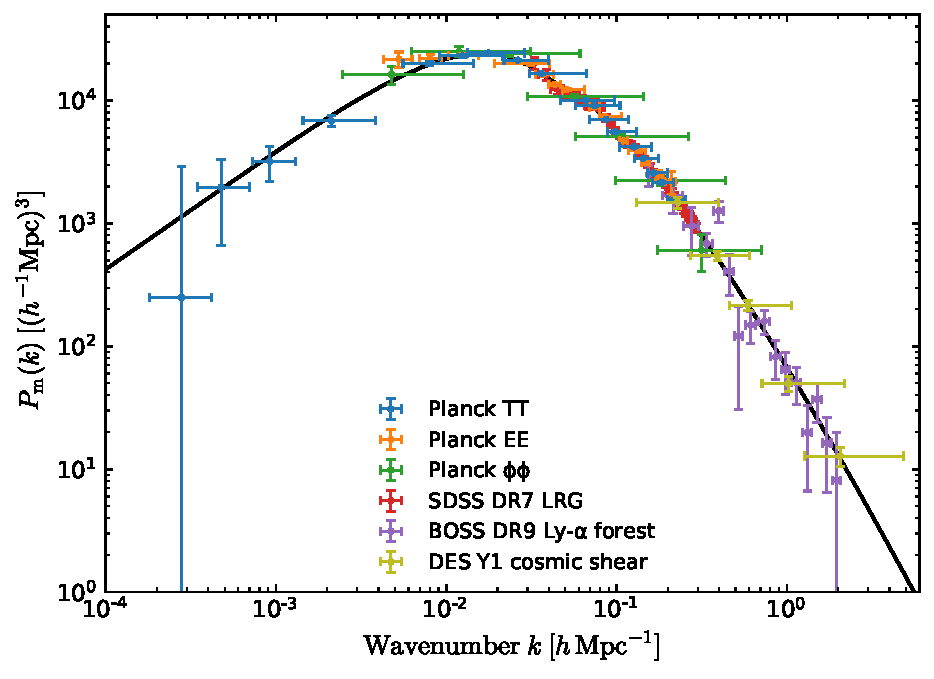
\includegraphics[width=0.8\textwidth]{img/matterpowerspectrum.pdf}
    \caption{Linear (total) matter power spectrum $P(k)$ versus wavenumber extrapolated to $z=0$ from various measurements of cosmological structure. The best fit $\Lambda$CDM model is shown as a solid line.}
    \label{fgr:matterpowerspectrum}
\end{figure}
\par The (total) matter power spectrum is significantly modified with respect to the original. The resulting $P(k)$ predicted by $\Lambda$CDM model is in very good agreement with observations.
\par Note that in the linear regime and matter domination the shape of $P(k)$ is (approximately) fixed, only the normalization changes.